\subsection{屈内特（Künneth）公式}

在本节中，我们考虑一个右 A-模的复形 (C, d) 和一个左 A-模的复形 (C', d')。考虑典范正合序列

\[
0 \rightarrow \mathrm{Z} (\mathrm{C}) \stackrel {{j}} {{\rightarrow}} \mathrm{C} \stackrel {{\delta}} {{\rightarrow}} \mathrm{B} (\mathrm{C}) (- 1) \rightarrow 0,\tag{I}
\]

\[
0 \rightarrow \mathrm{B} (\mathrm{C}) \xrightarrow {i} \mathrm{Z} (\mathrm{C}) \xrightarrow {p} \mathrm{H} (\mathrm{C}) \rightarrow 0;\tag{II}
\]

我们从 δ 推出一个 k-同态

\[
\mathrm{H} (\delta \otimes 1): \mathrm{H} (\mathrm{C} \otimes_ {\mathrm{A}} \mathrm{C} ^ {\prime}) \rightarrow \mathrm{H} (\mathrm{B} (\mathrm{C}) \otimes_ {\mathrm{A}} \mathrm{C} ^ {\prime}) (- 1);
\]

我们由(II)推出一个连接同态

\[
\partial (\mathrm{II}, \mathrm{H} (\mathrm{C} ^ {\prime})): \operatorname{Tor} _ {1} ^ {\mathbf {A}} (\mathrm{H} (\mathrm{C}), \mathrm{H} (\mathrm{C} ^ {\prime})) \rightarrow \mathrm{B} (\mathrm{C}) \otimes_ {\mathbf {A}} \mathrm{H} (\mathrm{C} ^ {\prime});
\]

如果我们装备 \(\operatorname{Tor}_{1}^{\mathbf{A}}(\mathrm{H}(\mathbf{C}),\mathrm{H}(\mathbf{C}^{\prime}))\) 其齐次分量的次数为 \(n\) 是 \(\bigoplus_{p+q=n}\operatorname{Tor}_{1}^{\mathbf{A}}(\mathrm{H}_{p}(\mathbf{C}),\mathrm{H}_{q}(\mathbf{C}^{\prime}))\) ，这个连接同态是次数为0的分次同态。此外，存在一个典范同态（X，第62页）

\[
\gamma (\mathrm{B} (\mathrm{C}), \mathrm{C} ^ {\prime}): \mathrm{B} (\mathrm{C}) \otimes_ {\mathrm{A}} \mathrm{H} (\mathrm{C} ^ {\prime}) \rightarrow \mathrm{H} (\mathrm{B} (\mathrm{C}) \otimes_ {\mathrm{A}} \mathrm{C} ^ {\prime}).
\]

在这些记号下：

定理3. --- 假设 A-模 B(C) 和 Z(C) 是平坦的。存在唯一的一个次数为 -1 的分次 k-模同态，

\[
\alpha : \mathrm{H} (\mathrm{C} \otimes_ {\mathrm{A}} \mathrm{C} ^ {\prime}) \rightarrow \operatorname{Tor} _ {1} ^ {\mathrm{A}} (\mathrm{H} (\mathrm{C}), \mathrm{H} (\mathrm{C} ^ {\prime}))
\]

从而使得图表交换

\[
\begin{array}{c} \mathrm{H} (\mathrm{C} \otimes_ {\mathrm{A}} \mathrm{C} ^ {\prime}) \xrightarrow {\alpha} \operatorname{Tor} _ {1} ^ {\mathrm{A}} (\mathrm{H} (\mathrm{C}), \mathrm{H} (\mathrm{C} ^ {\prime})) (- 1) \\ \mathrm{H} (\delta \otimes 1) \Biggl \downarrow \qquad \qquad \qquad \qquad \qquad \qquad \qquad \qquad \qquad \qquad \qquad \qquad \Biggl \downarrow \hat {c} (\Pi , \mathrm{H} (\mathrm{C} ^ {\prime})) \\ \mathrm{H} (\mathrm{B} (\mathrm{C}) \otimes_ {\mathrm{A}} \mathrm{C} ^ {\prime}) (- 1) \xleftarrow {\gamma (\mathrm{B} (\mathrm{C}) . \mathrm{C} ^ {\prime})} (\mathrm{B} (\mathrm{C}) \otimes_ {\mathrm{A}} \mathrm{H} (\mathrm{C} ^ {\prime})) (- 1). \end{array}
\]

分次k模的序列

\[
0 \longrightarrow \mathrm{H} (\mathrm{C}) \otimes_ {\mathrm{A}} \mathrm{H} \left(\mathrm{C} ^ {\prime}\right) \xrightarrow {\gamma \left(\mathrm{C} , \mathrm{C} ^ {\prime}\right)} \mathrm{H} \left(\mathrm{C} ^ {\prime} \otimes_ {\mathrm{A}} \mathrm{C} ^ {\prime}\right) \xrightarrow {\alpha} \operatorname{Tor} _ {1} ^ {\mathrm{A}} \left(\mathrm{H} (\mathrm{C}), \mathrm{H} \left(\mathrm{C} ^ {\prime}\right)\right) (- 1) \longrightarrow 0
\]

是正合的。

因此对每个 \( n \)，我们有一个正合序列

\[
\begin{array}{c} 0 \longrightarrow \bigoplus_ {p + q = n} \mathrm{H} _ {p} (\mathrm{C}) \otimes_ {\mathrm{A}} \mathrm{H} _ {q} (\mathrm{C} ^ {\prime}) \xrightarrow {\gamma_ {n} (\mathrm{C} , \mathrm{C} ^ {\prime})} \mathrm{H} _ {n} (\mathrm{C} \otimes_ {\mathrm{A}} \mathrm{C} ^ {\prime}) \\ \xrightarrow {\alpha_ {n}} \bigoplus_ {p + q = n - 1} \operatorname{Tor} _ {1} ^ {\mathrm{A}} \left(\mathrm{H} _ {p} (\mathrm{C}), \mathrm{H} _ {q} (\mathrm{C} ^ {\prime})\right) \longrightarrow 0. \end{array}\tag{11}
\]

为简单起见，设 \(\mathbf{B} = \mathbf{B}(\mathbf{C})\) , \(\mathbf{Z} = \mathbf{Z}(\mathbf{C})\) , \(\mathbf{H} = \mathbf{H}(\mathbf{C})\) 和 \(\mathbf{H}' = \mathbf{H}(\mathbf{C}')\)：

由于 B 是平坦的，我们从 (I) 推出一个正合序列（X，第 72 页，推论 2）

\[
0 \longrightarrow Z \otimes_ {A} C ^ {\prime} \xrightarrow {j \otimes 1} C \otimes_ {A} C ^ {\prime} \xrightarrow {\delta \otimes 1} (B \otimes_ {A} C ^ {\prime}) (- 1) \longrightarrow 0.\tag{12}
\]

引理 3. --- 与正合序列 (12) 相关联的连接同态 H(B ⊗\_A C') → H(Z ⊗\_A C') 等于 H(i ⊗ 1)。

事实上，设 \(a \in \mathbf{Z}(\mathbf{B} \otimes_{\mathbf{A}} \mathbf{C}')\) ；由于 B 是平坦的， \(a\) 属于 \(\mathbf{B} \otimes_{\mathbf{A}} \mathbf{Z}(\mathbf{C}')\) 的像，因此可以写成 \(\sum_{\lambda} da_{\lambda} \otimes b_{\lambda}\) ，具有 \(a_{\lambda} \in \mathbf{C}\) , \(b_{\lambda} \in \mathbf{C}'\) , \(db_{\lambda} = 0\) 。

\(a\) 的类在所求同态下的像按定义是 \(\mathbf{D}(\sum a_{\lambda}\otimes b_{\lambda})=\sum da_{\lambda}\otimes b_{\lambda}=(i\otimes1)(a)\) 的类，从而引理得证。

因此，与（12）相关联的同调正合列是

\[
\begin{array}{r l} \mathrm{H} (\mathrm{B} \otimes_ {\mathrm{A}} \mathrm{C} ^ {\prime}) & \xrightarrow {\mathrm{H} (i \otimes 1)} \mathrm{H} (\mathrm{Z} \otimes_ {\mathrm{A}} \mathrm{C} ^ {\prime}) \xrightarrow {\mathrm{H} (j \otimes 1)} \mathrm{H} (\mathrm{C} \otimes_ {\mathrm{A}} \mathrm{C} ^ {\prime}) \\ & \xrightarrow {\mathrm{H} (\delta \otimes 1)} \mathrm{H} (\mathrm{B} \otimes_ {\mathrm{A}} \mathrm{C} ^ {\prime}) (- 1) \xrightarrow {\mathrm{H} (i \otimes 1)} \mathrm{H} (\mathrm{Z} \otimes_ {\mathrm{A}} \mathrm{C} ^ {\prime}) (- 1). \end{array}
\]

此外，由于Z是平坦的，我们从(II)推出一个分次k-模的正合序列

\[
0 \longrightarrow \operatorname{Tor} _ {1} ^ {\mathrm{A}} (\mathrm{H}, \mathrm{H} ^ {\prime}) \xrightarrow {\hat {c} (\mathrm{II} , \mathrm{H} ^ {\prime})} \mathrm{B} \otimes_ {\mathrm{A}} \mathrm{H} ^ {\prime} \xrightarrow {i \otimes 1} Z \otimes_ {\mathrm{A}} \mathrm{H} ^ {\prime} \xrightarrow {p \otimes 1} \mathrm{H} \otimes_ {\mathrm{A}} \mathrm{H} ^ {\prime} \longrightarrow 0;
\]

最后，我们有第1号中的典范同态

\[
\gamma_ {\mathbf {B}} = \gamma (\mathbf {B}, \mathbf {C} ^ {\prime}): \mathbf {B} \otimes_ {\mathbf {A}} \mathrm{H} ^ {\prime} \rightarrow \mathrm{H} (\mathbf {B} \otimes_ {\mathbf {A}} \mathbf {C} ^ {\prime})
\]

\[
\gamma_ {Z} = \gamma (Z, C ^ {\prime}): Z \otimes_ {A} H ^ {\prime} \rightarrow H (Z \otimes_ {A} C ^ {\prime})
\]

\[
\gamma_ {\mathrm{C}} = \gamma (\mathrm{C}, \mathrm{C} ^ {\prime}): \mathrm{H} \otimes_ {\mathrm{A}} \mathrm{H} ^ {\prime} \rightarrow \mathrm{H} (\mathrm{C} \otimes_ {\mathrm{A}} \mathrm{C} ^ {\prime}),
\]

由此得到一个分次k-模的图表，其行是正合的

\[
\begin{array}{r l} & \mathbf {B} \otimes \mathbf {H} ^ {\prime} \xrightarrow [ \gamma_ {B} ]{i \otimes 1} \mathbf {Z} \otimes \mathbf {H} ^ {\prime} \xrightarrow [ \gamma_ {Z} ]{p \otimes 1} \mathbf {H} \otimes \mathbf {H} ^ {\prime} \longrightarrow 0 \\ & \mathrm{H} (\mathbf {B} \otimes \mathbf {C} ^ {\prime}) \xrightarrow {\mathrm{H} (i \otimes 1)} \mathrm{H} (\mathbf {Z} \otimes \mathbf {C} ^ {\prime}) \xrightarrow {\mathrm{H} (j \otimes 1)} \mathrm{H} (\mathbf {C} \otimes \mathbf {C} ^ {\prime}) \xrightarrow {\mathrm{H} (\delta \otimes 1)} \mathrm{H} (\mathbf {B} \otimes \mathbf {C} ^ {\prime}) (- 1) \xrightarrow {\mathrm{H} (i \otimes 1)} \mathrm{H} (\mathbf {Z} \otimes \mathbf {C} ^ {\prime}) (- 1) \\ & 0 \longrightarrow \operatorname{Tor} _ {1} ^ {\mathrm{A}} (\mathrm{H}, \mathrm{H} ^ {\prime}) (- 1) \xrightarrow {\delta (\mathrm{II.H} ^ {\prime})} (\mathbf {B} \otimes \mathbf {H} ^ {\prime}) (- 1) \xrightarrow [ i \otimes 1 ]{\gamma_ {B}} (\mathbf {Z} \otimes \mathbf {H} ^ {\prime}) (- 1), \end{array}
\]

这由同态 \(\gamma\) 的定义是交换的。但是，由于复形 B 和 Z 是分裂且平坦的， \(\gamma_{\mathbf{B}}\) 和 \(\gamma_{\mathbf{Z}}\) 是双射的（X，第 65 页，推论 1）。由此一方面可推出， \(\gamma_{\mathbf{C}}\) 是单射，其像等于 Ker H( \(\delta \otimes 1\) )，另一方面， \(\gamma_{\mathbf{B}} \circ \partial(\mathrm{II}, \mathrm{H}')\) 是单射，其像等于 Im H( \(\delta \otimes 1\) )。定理由此直接得出。

推论1. --- 若B(C)和Z(C)是平坦的，则对每个左A模N和每个整数n，存在一个正合序列

\[
0 \longrightarrow \mathrm{H} _ {n} (\mathrm{C}) \otimes_ {\mathrm{A}} \mathrm{N} \xrightarrow {\gamma_ {n}} \mathrm{H} _ {n} (\mathrm{C} \otimes_ {\mathrm{A}} \mathrm{N}) \xrightarrow {\alpha_ {n}} \operatorname{Tor} _ {1} ^ {\mathrm{A}} \left(\mathrm{H} _ {n - 1} (\mathrm{C}), \mathrm{N}\right) \longrightarrow 0.\tag{13}
\]

推论2.——设 B(C) 和 B(C') 是投射的，且 Z(C) 是平坦的。则 k-模序列 (11) 和 (13) 是正合且分裂的。

这由定理及以下引理得出：

引理4. --- 若 B(C) 和 B(C') 是投射的，则典范同态

\[
\gamma (\mathbf {C}, \mathbf {C} ^ {\prime}): \mathrm{H} (\mathbf {C}) \otimes_ {\mathbf {A}} \mathrm{H} (\mathbf {C} ^ {\prime}) \rightarrow \mathrm{H} (\mathbf {C} \otimes_ {\mathbf {A}} \mathbf {C} ^ {\prime})
\]

有一个 k-线性收缩。

事实上，根据 X，第 65 页，注记 b)，存在拟同构 \(\varphi: C \to H(C)\) 和 \(\varphi': C' \to H(C')\) 使得 \(H(\varphi) = 1_{H(C)}\) 和 \(H(\varphi') = 1_{H(C')}\) 。在交换图中

\[
\begin{array}{c} \mathrm{H(C)} \otimes_ {\mathrm{A}} \mathrm {H(C^ {\prime})} \xrightarrow {\gamma (\mathrm{C,C} ^ {\prime})} \mathrm {H(C} \otimes_ {\mathrm{A}} \mathrm {C^ {\prime})} \\ \mathrm {H}(\varphi) \otimes \mathrm {H}(\varphi^ {\prime}) \Big \downarrow \\ \mathrm {H(C)} \otimes_ {\mathrm{A}} \mathrm {H(C^ {\prime})} \xrightarrow {\gamma (\mathrm{H(C),H(C^ {\prime})})} \mathrm {H(C)} \otimes_ {\mathrm{A}} \mathrm {H(C^ {\prime})} \end{array}
\]

\(\mathrm{H}(\varphi) \otimes \mathrm{H}(\varphi') \text{ 和 } \gamma(\mathrm{H}(\mathrm{C}), \mathrm{H}(\mathrm{C}') ) \text{ 是恒等映射，由此得出断言。}\)

推论3（“泛系数公式”）。—— 设环 A 是主理想环。若复形 C 与 C' 是自由的，则 A-模序列 (11) 是正合且分裂的；若复形 C 是自由的，则对每个 A-模 N，A-模序列 (13) 是正合且分裂的。

事实上，B(C)、Z(C) 和 B(C') 是自由模 C、C、C' 的子模，因此是自由的（VII，§3，定理1的推论2），于是应用推论2。

推论4（“屈内特公式”）。——设 C 上有界，且 C 与 H(C) 是平坦的；则典范同态

\[
\gamma (\mathrm{C}, \mathrm{C} ^ {\prime}): \mathrm{H} (\mathrm{C}) \otimes_ {\mathrm{A}} \mathrm{H} (\mathrm{C} ^ {\prime}) \rightarrow \mathrm{H} (\mathrm{C} \otimes_ {\mathrm{A}} \mathrm{C} ^ {\prime})
\]

是双射。

由该定理，只需证明 B(C) 和 Z(C) 是平坦的。现在我们有以下正合序列

\[
0 \to \mathrm{B} _ {n} (\mathrm{C}) \to \mathrm{Z} _ {n} (\mathrm{C}) \to \mathrm{H} _ {n} (\mathrm{C}) \to 0
\]

\[
0 \to Z _ {n} (\mathbf {C}) \to \mathbf {C} _ {n} \to \mathbf {B} _ {n - 1} (\mathbf {C}) \to 0,
\]

由此，根据 X 第 75 页推论 1，可得如下蕴含关系 \((\mathbf{B}_{n-1}(\mathbf{C})\) 是平坦的) \(\Rightarrow (\mathbf{Z}_n(\mathbf{C})\) 是平坦的) \(\Rightarrow (\mathbf{B}_n(\mathbf{C})\) 是平坦的)；我们注意到 \(\mathbf{B}_n(\mathbf{C}) = 0\) 对足够小的 \(n\) 成立，由此得出结论。

推论5. --- 设 \(u: \mathbf{C} \to \mathbf{C}'\) 为右 A-模复形的同态，平坦且右有界。对于左 A-模的每个复形 E，态射 \(u \otimes 1_{\mathbf{E}}: \mathbf{C} \otimes_{\mathbf{A}} \mathbf{E} \to \mathbf{C}' \otimes_{\mathbf{A}} \mathbf{E}\) 是拟同构。

确实，Con \((u)\) 是一个平坦复形，右有界且同调为零；因此由推论4，我们有 H(Con \((u) \otimes_{\mathbf{A}} \mathbf{E}) = 0\) ，故 H(Con \((u \otimes 1_{\mathbf{E}})) = 0\) （X，第 67 页，引理2），从而 \(u \otimes 1_{\mathbf{E}}\) 是拟同构。

\subsection{诺特环上的有界平坦复形}

命题11。——设 A 是左诺特环，令 C 为平坦左 A-模的有界复形，且 H(C) 是有限生成 A-模。设 a 和 b 为两个整数，使得 \(a \leqslant b\) 并且 \(\mathrm{H}_{n}(\mathrm{C}) = 0\) （当 \(n < a\) ）， \(\mathrm{C}_{n} = 0\) （当 \(n > b\) ）。存在一个左 A-模复形 P，使得 \(\mathrm{P}_{n}\) 对每个 \(n\) 都是投射且有限生成的，并且 \(\mathrm{P}_{n} = 0\) （当 \(n \notin [a, b]\) ），以及一个拟同构 \(u: \mathrm{P} \to \mathrm{C}\) 。此外，对于右 A-模的每个复形 E，同态

\[
\mathrm{H} \left(1 _ {\mathrm{E}} \otimes u\right): \mathrm{H} (\mathrm{E} \otimes_ {\mathrm{A}} \mathrm{P}) \rightarrow \mathrm{H} (\mathrm{E} \otimes_ {\mathrm{A}} \mathrm{C}) \quad \text{是双射。}
\]

根据 X，第 53 页，命题 7，存在一个复形 (L, d)，使得 \(L_{n}\) 对每个 n 都是自由且有限生成的，并且当 n \textless{} a 时为零，以及一个拟同构 \(f: L \to C\) 。设 P 为商复形 \(L/L'\) ，其中 \(L_{n}' = 0\) （当 n \textless{} b ）， \(L_{n}' = L_{n}\) （当 n \textgreater{} b ），以及 \(L_{b}' = B_{b}(L)\) 。由于 \(C_{n} = 0\) （当 n \textgreater{} b ），故 \(f(L') = 0\) ，因此 f 通过一个复形态射 \(u: P \to C\) 分解.

\[
\begin{array}{c c c c c} \dots \longrightarrow & L _ {b + 1} & \xrightarrow {d _ {b + 1}} & L _ {b} & \xrightarrow {d _ {b}} L _ {b - 1} \longrightarrow \dots \\ & \downarrow & & \downarrow & | | \\ & 0 & \longrightarrow & P _ {b} & \longrightarrow P _ {b - 1} \longrightarrow \dots \\ & \downarrow & & \downarrow^ {u _ {b}} & \downarrow^ {u _ {b - 1}} \\ & 0 & \longrightarrow & C _ {b} & \longrightarrow C _ {b - 1} \longrightarrow \dots \end{array}
\]

由于 \(f\) 是一个拟同构，我们有 \(\mathrm{H}(\mathrm{Con}(f)) = 0\) ，由此得到正合序列

\[
\dots \rightarrow \mathrm{L} _ {b + 1} \xrightarrow {d _ {b + 1}} \mathrm{L} _ {b} \longrightarrow \mathrm{L} _ {b - 1} \oplus \mathrm{C} _ {b} \longrightarrow \mathrm{L} _ {b - 2} \oplus \mathrm{C} _ {b - 1} \rightarrow \dots .
\]

因此我们有一个正合序列

\[
0 \rightarrow \mathrm{P} _ {b} \rightarrow \mathrm{L} _ {b - 1} \oplus \mathrm{C} _ {b} \rightarrow \mathrm{L} _ {b - 2} \oplus \mathrm{C} _ {b - 1} \rightarrow \dots .
\]

这表明，一方面， \(u\) 的锥体具有零同调，因此 \(u\) 是拟同构，另一方面，模 \(\mathbf{P}_{b}\) 是平坦的（X，第 76 页，推论2）；由于 \(\mathbf{P}_{b}\) 作为 \(\mathbf{L}_{b+1}\) 的商是有限型的，它是投射的（X，第 13 页，推论）。因此，数对 (P, u) 满足所需条件。最后一个断言由 X，第 79 页，推论 5 得出。

* 例。--- 设 A 为诺特交换环，X 为 A 上的真且平坦的概形， \(\mathcal{F}\) 为一个凝聚 \(\mathcal{O}_{\mathbf{X}}\)-模，在 A 上平坦。存在一个有界复形 P，由有限生成的投射 A-模组成，使得对每个 A-模 M，H(X, \(\mathcal{F} \otimes_{\mathbf{A}} \mathbf{M}\) ) 自然等同于 H(P \(\otimes_{\mathbf{A}} \mathbf{M}\) ) 。事实上，设 \(\mathfrak{U}\) 为 X 的由有限个仿射开集组成的覆盖， \(\mathcal{E}(\mathfrak{U}, \mathcal{F})\) 为相应的 Čech 复形：可证明 H \(^{i}\) ( \(\mathcal{E}(\mathfrak{U}, \mathcal{F})\) ) 同构于 A-模 H \(^{i}\) (X, \(\mathcal{F}\) ) ，且后者是有限生成的；此外，对每个 A-模 M，复形 \(\mathcal{E}(\mathfrak{U}, \mathcal{F}) \otimes_{\mathbf{A}} \mathbf{M}\) 同构于 \(\mathcal{E}(\mathfrak{U}, \mathcal{F} \otimes_{\mathbf{A}} \mathbf{M})\) 。将命题11应用于复形 \(\mathcal{E}(\mathfrak{U}, \mathcal{F})\) （它是有界的），得到一个满足要求的复形 P。

设 \(y\) 为 \(\text{Spec}(\mathbf{A})\) 的一点， \(\kappa(y)\) 为 \(\mathbf{A}\) 在 \(y\) 的剩余域， \(X_y = X \otimes_{\mathbf{A}} \kappa(y)\) 为 \(\mathbf{X}\) 在 \(y\) 之上的纤维， \(\mathcal{F}_y = \mathcal{F} \otimes_{\mathbf{A}} \kappa(y)\) ，并令 \(h^p(y) = \dim_{\kappa(y)} H^p(X_y, \mathcal{F}_y)\) （当 \(p \geqslant 0\) ）。由复形 \(\mathbf{P}\) 的存在性容易推出以下结果：

\begin{enumerate}
\def\labelenumi{(\roman{enumi})}
\item
  函数 \(h^{p}\) 在 Spec(A) 上是上半连续的；
\item
  函数 \(\sum_{p\geqslant 0}(-1)^{p}h^{p}\) 在 \(\operatorname {Spec}(\mathbf{A})\) 上是局部常数的.*
\end{enumerate}

\subsection{推广到多模复形}

设 B 和 B' 为两个环，C 为 (B, A)-双模复形，C' 为 (A, B')-双模复形（X，第 43 页）；则 (C ⊗\_A C', D) （X，第 61 页）是 (B, B')-双模的复形，且典范同态

\[
\gamma : \mathrm{H} (\mathbf {C}) \otimes_ {\mathbf {A}} \mathrm{H} (\mathbf {C} ^ {\prime}) \rightarrow \mathrm{H} (\mathbf {C} \otimes_ {\mathbf {A}} \mathbf {C} ^ {\prime})
\]

与两个成员的(B, B')-双模结构相容。

若 B'' 是第三个环，且 C'' 是 (B', B'')-双模的复形，则典范同态（II，第 64 页，命题 8）

\[
\left(\mathrm{C} \otimes_ {\mathrm{A}} \mathrm{C} ^ {\prime}\right) \otimes_ {\mathrm{B} ^ {\prime}} \mathrm{C} ^ {\prime \prime} \rightarrow \mathrm{C} \otimes_ {\mathrm{A}} \left(\mathrm{C} ^ {\prime} \otimes_ {\mathrm{B} ^ {\prime \prime}} \mathrm{C} ^ {\prime \prime}\right)
\]

是(B, B'')-双模复形的一个同构。

更一般地，我们留给读者按照第 1 号（X，第 63 页）以及 II，第 65 至 72 页的模型，发展有限全序族多模复形的张量积理论（结合性与交换性同构， \ldots).

设 B 和 B′ 为两个环，M 为 (B, A)-双模，N 为 (A, B′)-双模：则 L(M) ⊗\_A L(N) 是 (B, B')-双模的复形，因此 Tor\^{}A (M, N) 具有自然的 (B, B')-双模分次结构；在 0 次项上，该结构与 M ⊗\_A N 的结构一致。

若 \(\lambda\in\mathbf{B},\lambda^{\prime}\in\mathbf{B}^{\prime}\) ，且若我们记 \(\lambda_{\mathbf{M}},\lambda_{\mathbf{N}}^{\prime},\lambda_{\mathbf{T}},\lambda_{\mathbf{T}}^{\prime}\) 为位似 \(x\mapsto\lambda x,y\mapsto y\lambda^{\prime},z\mapsto\lambda z,z\mapsto z\lambda^{\prime}\) ，它们分别作用于 \(\mathbf{M},\mathbf{N},\mathrm{Tor}^{\mathbf{A}}(\mathbf{M},\mathbf{N}),\mathrm{Tor}^{\mathbf{A}}(\mathbf{M},\mathbf{N})\) ，则

\[
\lambda_ {\mathrm{T}} = \operatorname{Tor} ^ {\mathbf {A}} \left(\lambda_ {\mathbf {M}}, 1 _ {\mathbf {N}}\right), \quad \lambda_ {\mathrm{T}} ^ {\prime} = \operatorname{Tor} ^ {\mathbf {A}} \left(1 _ {\mathbf {M}}, \lambda_ {\mathbf {N}} ^ {\prime}\right),
\]

这给出了Tor \(^{A}\) (M, N)双模结构的另一种描述。我们留给读者将第5号和第7号推广到多模复形的情形。

\section{扩张模}

我们沿用§4的一般记号。此外约定，除非另有明确说明，所考虑的所有模均为左模，所考虑的所有复形均为左模复形。

\subsection{同态复形}

设 (C, d) 和 (C', d') 是两个 A-复形。考虑分次 k-模 Homgr\_A(C, C')（II，第 174–175 页）：对于 \(n \in \mathbf{Z}\) ，Homgr\_A(C, C')\_n 是从 C 到 C' 的、次数为 \(n\) 的 A-线性分次映射所成的 k-模；换言之，Homgr\_A(C, C') 与 A-模典范地等同

\[
\bigoplus_ {n \in \mathbf {Z}} \prod_ {p \in \mathbf {Z}} \operatorname{Hom} _ {\mathrm{A}} \left(\mathrm{C} _ {p}, \mathrm{C} _ {p + n} ^ {\prime}\right) = \bigoplus_ {n \in \mathbf {Z}} \prod_ {p + q = n} \operatorname{Hom} _ {\mathrm{A}} \left(\mathrm{C} _ {p}, \mathrm{C} ^ {\prime q}\right).
\]

我们来定义 k-线性映射：

\[
\mathrm{D} _ {n}: \operatorname{Homgr} _ {\mathbf {A}} (\mathrm{C}, \mathrm{C} ^ {\prime}) _ {n} \rightarrow \operatorname{Homgr} _ {\mathbf {A}} (\mathrm{C}, \mathrm{C} ^ {\prime}) _ {n - 1}, \quad n \in \mathbf {Z},
\]

如下

\[
\mathbf {D} _ {n} (f) = d ^ {\prime} \circ f - (- 1) ^ {n} f \circ d;\tag{1}
\]

我们有

\[
\begin{array}{r l} \mathrm{D} _ {n - 1} \circ \mathrm{D} _ {n} (f) = & \mathrm{D} _ {n - 1} \left(d ^ {\prime} \circ f - (- 1) ^ {n} f \circ d\right) = d ^ {\prime} \circ d ^ {\prime} \circ f - (- 1) ^ {n} d ^ {\prime} \circ f \circ d \\ & - (- 1) ^ {n - 1} d ^ {\prime} \circ f \circ d - f \circ d \circ d = 0. \end{array}
\]

则 (Homgr \(_{A}\) (C, C'), D) 是一个 \(k\) -模复形，称为从 C 到 C' 的同态复形。

例如， \(\operatorname{Homgr}_{\mathbf{A}}(\mathbf{A}, \mathbf{C}')\) 与 \(\mathbf{C}'\) 典范地等同。我们还注意到，对于每一个 \(n \in \mathbf{Z}\) ，有 \(\operatorname{Homgr}_{\mathbf{A}}(\mathbf{C}, \mathbf{C}')\) ( \(n\) ) = \(\operatorname{Homgr}_{\mathbf{A}}(\mathbf{C}, \mathbf{C}'(n))\) .

\(Z_n(\text{Homgr}_A(C, C'))\) 的元素是这样的分次同态 \(f\) ：次数为（下降） \(n\) ，从 \(C\) 到 \(C'\) ，且满足 \(d' \circ f = (-1)^n f \circ d\) ，即从 \(C\) 到 \(C'(n)\) 的复形态射，或再次为从 \(C(p)\) 到 \(C'(p + n)\) （对任意固定的 \(p\) ）的复形态射。它们称为（下降）次数为 \(n\) 的、从 \(C\) 到 \(C'\) 的复形态射；若 \(f, g \in Z_n(\text{Homgr}_A(C, C'))\) 和 \(s \in \text{Homgr}_A(C, C')_{n+1}\) ，则条件 \(g - f = Ds\) 意味着 \(s\) 是连接态射 \(f\) 和 \(g\) （从 \(C\) 到 \(C'(n)\) ）的同伦，从而 \(H_n(\text{Homgr}_A(C, C'))\) 是 \(k\) -模，它由（下降）次数为 \(n\) 的、从 \(C\) 到 \(C'\) 的态射的同伦类组成.

设 \(\alpha\in\mathrm{H}_{n}(\mathrm{Homgr}_{\mathrm{A}}(\mathrm{C},\mathrm{C}^{\prime}))\) 和 \(p\in\mathbf{Z}\) 。令 \(\alpha\) 由 \(f\in\mathbf{Z}_{n}(\mathrm{Homgr}_{\mathrm{A}}(\mathrm{C},\mathrm{C}^{\prime}))\) 代表；则 \(f\) 是从 \(\mathbf{C}\) 到 \(\mathbf{C}^{\prime}(n)\) 的复形态射，因此 \(\mathbf{H}_{p}(f)\) 是从 \(\mathbf{H}_{p}(\mathbf{C})\) 到 \(\mathbf{H}_{p}(\mathbf{C}^{\prime}(n))=\mathbf{H}_{p+n}(\mathbf{C}^{\prime})\) 的同态；由于 \(\mathbf{H}_{p}(f)\) 仅依赖于同伦类 \(\alpha\) （ \(f(\mathbf{X},\mathbf{p.~33,~prop.~3})\) ） ，我们推出一个典范的 \(k\) -模同态

\[
\mathrm{H} _ {n} \left(\operatorname{Homgr} _ {\mathrm{A}} \left(\mathrm{C}, \mathrm{C} ^ {\prime}\right)\right)\rightarrow \operatorname{Hom} _ {\mathrm{A}} \left(\mathrm{H} _ {p} (\mathrm{C}), \mathrm{H} _ {p + n} \left(\mathrm{C} ^ {\prime}\right)\right),
\]

由此得到一个次数为0的分次k-线性映射，称为典范映射

\[
\lambda (\mathrm{C}, \mathrm{C} ^ {\prime}): \mathrm{H} (\operatorname{Homgr} _ {\mathbf {A}} (\mathrm{C}, \mathrm{C} ^ {\prime})) \rightarrow \dot {\operatorname{Homgr}} _ {\mathbf {A}} (\mathrm{H} (\mathrm{C}), \mathrm{H} (\mathrm{C} ^ {\prime})).
\]

\(\lambda(C, C')\) 的分次分量通常记作：

\[
\lambda^ {n} (\mathrm{C}, \mathrm{C} ^ {\prime}): \mathrm{H} ^ {n} \left(\operatorname{Homgr} _ {\mathrm{A}} \left(\mathrm{C}, \mathrm{C} ^ {\prime}\right)\right)\rightarrow \prod_ {p + q = n} \operatorname{Hom} _ {\mathrm{A}} \left(\mathrm{H} _ {p} (\mathrm{C}), \mathrm{H} ^ {q} \left(\mathrm{C} ^ {\prime}\right)\right).
\]

命题1. — 若 C 右零且 C' 左零，则 Homgr \(_{A}\) (C, C') 左零，且典范 k-线性映射

\[
\lambda^ {0} (\mathrm{C}, \mathrm{C} ^ {\prime}): \mathrm{H} ^ {0} \left(\operatorname{Homgr} _ {\mathrm{A}} (\mathrm{C}, \mathrm{C} ^ {\prime})\right)\rightarrow \operatorname{Hom} _ {\mathrm{A}} \left(\mathrm{H} _ {0} (\mathrm{C}), \mathrm{H} ^ {0} \left(\mathrm{C} ^ {\prime}\right)\right)
\]

是双射。

我们有正合序列

\[
0 \longrightarrow \mathrm{H} ^ {0} (\mathrm{C} ^ {\prime}) \stackrel {i} {\longrightarrow} \mathrm{C} ^ {\prime 0} \stackrel {d ^ {\prime 0}} {\longrightarrow} \mathrm{C} ^ {\prime 1}
\]

\[
\mathrm{C} _ {1} \xrightarrow {d _ {1}} \mathrm{C} _ {0} \xrightarrow {p} \mathrm{H} _ {0} (\mathrm{C}) \longrightarrow 0.
\]

另一方面， \(\mathrm{Homgr}_{\mathbf{A}}^{0}(\mathbf{C},\mathbf{C}^{\prime})\) 等同于 \(\mathrm{Hom}_{\mathbf{A}}(\mathbf{C}_{0},\mathbf{C}^{\prime 0})\) ，而 \(\mathbf{Z}^{0}(\mathrm{Homgr}_{\mathbf{A}}(\mathbf{C},\mathbf{C}^{\prime}))\) 则等同于这样的 \(f:\mathbf{C}_{0}\to \mathbf{C}^{\prime 0}\) 所成的集合：它使得 \(d^{\prime 0}\circ f = 0\) , \(f\circ d_{1} = 0\) ； \(\mathbf{B}^{0}(\mathrm{Homgr}_{\mathbf{A}}(\mathbf{C},\mathbf{C}^{\prime}))\) 为零；最后，映射 \(\lambda^0\) 把 \(f\) 模 \(\{0\}\) 的类对应到同态 \(\varphi :\mathrm{H}_0(\mathrm{C})\to \mathrm{H}^0 (\mathrm{C}')\) （它使得 \(f = i\circ \varphi \circ p\) ），由此得出该命题。

设 \(u: \tilde{\mathbf{C}} \to \mathbf{C}\) 和 \(u': \mathbf{C}' \to \tilde{\mathbf{C}}'\) 是复形的态射；则典范同态 \(\operatorname{Homgr}_{\mathbf{A}}(u, u') : \operatorname{Homgr}_{\mathbf{A}}(\mathbf{C}, \mathbf{C}') \to \operatorname{Homgr}_{\mathbf{A}}(\tilde{\mathbf{C}}, \tilde{\mathbf{C}}')\) ，定义为 \(f\mapsto u^{\prime}\circ f\circ u\) 是复形的态射，这由公式（1）立即得出。此外，下面的图表是交换的

\[
\begin{array}{c} \mathrm{H} (\mathrm{Homgr} _ {\mathsf {A}} (\mathrm{C}, \mathrm{C} ^ {\prime})) \xrightarrow {\lambda (\mathrm{C} , \mathrm{C} ^ {\prime})} \mathrm{Homgr} _ {\mathsf {A}} (\mathrm{H} (\mathrm{C}), \mathrm{H} (\mathrm{C} ^ {\prime})) \\ \mathrm{H} (\mathrm{Homgr} _ {\mathsf {A}} (u, u ^ {\prime})) \Big \downarrow \\ \mathrm{H} (\mathrm{Homgr} _ {\mathsf {A}} (\tilde {\mathsf {C}}, \tilde {\mathsf {C}} ^ {\prime})) \xrightarrow {\lambda (\tilde {\mathsf {C}} , \tilde {\mathsf {C}} ^ {\prime})} \mathrm{Homgr} _ {\mathsf {A}} (\mathrm{H} (\tilde {\mathsf {C}}), \mathrm{H} (\tilde {\mathsf {C}} ^ {\prime}))  . \end{array}
\]

命题2. --- a) 设 \(C' \xrightarrow{u} C \xrightarrow{v} C''\) 是 A-复形的正合序列， \(P\) 是投射复形，E 是内射复形（X，第 25 页）。则序列

\[
\operatorname{Homgr} _ {\mathbf {A}} (\mathrm{P}, \mathrm{C} ^ {\prime}) \xrightarrow {\operatorname{Homgr} (1 , u)} \operatorname{Homgr} _ {\mathbf {A}} (\mathrm{P}, \mathrm{C}) \xrightarrow {\operatorname{Homgr} (1 , v)} \operatorname{Homgr} _ {\mathbf {A}} (\mathrm{P}, \mathrm{C} ^ {\prime \prime})
\]

和

\[
\operatorname{Homgr} _ {\mathbf {A}} \left(\mathrm{C} ^ {\prime \prime}, \mathrm{E}\right) \xrightarrow {\operatorname{Homgr} (v , 1)} \operatorname{Homgr} _ {\mathbf {A}} (\mathrm{C}, \mathrm{E}) \xrightarrow {\operatorname{Homgr} (u , 1)} \operatorname{Homgr} _ {\mathbf {A}} \left(\mathrm{C} ^ {\prime}, \mathrm{E}\right)
\]

是k-模复形的正合序列。

\begin{enumerate}
\def\labelenumi{\alph{enumi})}
\setcounter{enumi}{1}
\tightlist
\item
  设 \(0 \to \mathbf{C}' \xrightarrow{u} \mathbf{C} \xrightarrow{v} \mathbf{C}'' \to 0\) 是 A-复形的序列，它作为分次 A-模的正合序列是分裂的（例如，当 \(\mathbf{C}'\) 是内射的，或 \(\mathbf{C}''\) 是投射的时，即为这种情况）。则对每个复形 E，序列
\end{enumerate}

\[
0 \rightarrow \operatorname{Homgr} _ {\mathbf {A}} (\mathrm{E}, \mathrm{C} ^ {\prime}) \xrightarrow {\operatorname{Homgr} (1 , u)} \operatorname{Homgr} _ {\mathbf {A}} (\mathrm{E}, \mathrm{C}) \xrightarrow {\operatorname{Homgr} (1 , v)} \operatorname{Homgr} _ {\mathbf {A}} (\mathrm{E}, \mathrm{C} ^ {\prime \prime}) \rightarrow 0
\]

\[
0 \rightarrow \operatorname{Homgr} _ {\mathbf {A}} \left(\mathrm{C} ^ {\prime \prime}, \mathrm{E}\right) \xrightarrow {\operatorname{Homgr} (v , 1)} \operatorname{Homgr} _ {\mathbf {A}} (\mathrm{C}, \mathrm{E}) \xrightarrow {\operatorname{Homgr} (u , 1)} \operatorname{Homgr} _ {\mathbf {A}} \left(\mathrm{C} ^ {\prime}, \mathrm{E}\right)\rightarrow 0
\]

是k-模复形的正合序列。

在情形 \(a\) )，我们注意到序列

\[
\operatorname{Hom} _ {\mathbf {A}} \left(\mathrm{P} _ {p}, \mathrm{C} _ {q} ^ {\prime}\right)\rightarrow \operatorname{Hom} _ {\mathbf {A}} \left(\mathrm{P} _ {p}, \mathrm{C} _ {q}\right)\rightarrow \operatorname{Hom} _ {\mathbf {A}} \left(\mathrm{P} _ {p}, \mathrm{C} _ {q} ^ {\prime \prime}\right)
\]

和

\[
\operatorname{Hom} _ {\mathbf {A}} \left(\mathrm{C} _ {q} ^ {\prime \prime}, \mathrm{E} _ {p}\right)\rightarrow \operatorname{Hom} _ {\mathbf {A}} \left(\mathrm{C} _ {q}, \mathrm{E} _ {p}\right)\rightarrow \operatorname{Hom} _ {\mathbf {A}} \left(\mathrm{C} _ {q} ^ {\prime}, \mathrm{E} _ {p}\right)
\]

对所有 \(p, q \in \mathbf{Z}\) 都是正合的，并且我们应用 II，第 10 页，命题 5 以及 II，第 13 页，命题 7。 \(b\) ) 的证明是类似的。

\subsection{同态与同伦的复形}

命题3. --- 设 C， \(\tilde{C}\) , \(C'\) , \(\tilde{C}'\) 为四个 A-复形， \(u: \tilde{C} \to C\) , \(v: \tilde{C} \to C\) , \(u': C' \to \tilde{C}'\) 和 \(v': C' \to \tilde{C}'\) 为四个复形态射。

\begin{enumerate}
\def\labelenumi{\alph{enumi})}
\item
  如果 u 和 \(u'\) 分别与 v 和 \(v'\) 同伦，则这两个态射 \(\operatorname{Homgr}_{\mathbf{A}}(u, u')\) 和 \(\operatorname{Homgr}_{\mathbf{A}}(v, v')\) （从 \(\operatorname{Homgr}_{\mathbf{A}}(\mathbf{C}, \mathbf{C}')\) 到 \(\operatorname{Homgr}_{\mathbf{A}}(\tilde{\mathbf{C}}, \tilde{\mathbf{C}}')\) ）是同伦的。
\item
  如果 u 和 u' 是同伦等价，Homgr\_A(u, u') 是一个同伦等价。
\item
  如果 C 或 C' 同伦于零，则 Homgr\_A(C, C') 同伦于零。
\end{enumerate}

我们用同一个字母 \(d\) 表示复形 C, C \(_{1}\) ，C \(^{\prime}\) ，C \(_{1}^{\prime}\) 的微分，并用 D 表示 Homgr \(_{A}\) (C, C') 和 Homgr \(_{A}\) (C \(_{1}\) ，C \(_{1}^{\prime}\) ) 的微分。若 \(u\) （相应地， \(u^{\prime}\) ）同伦于 \(v\) （相应地， \(v^{\prime}\) ），则存在一个次数为 1 的分次同态，

\[
w: \mathrm{C} _ {1} \rightarrow \mathrm{C} \quad (\text { resp. } w ^ {\prime}: \mathrm{C} ^ {\prime} \rightarrow \mathrm{C} _ {1} ^ {\prime})
\]

使得

\[
u - v = d w + w d \quad (\text { resp. } u ^ {\prime} - v ^ {\prime} = d w ^ {\prime} + w ^ {\prime}\tag{2}
\]

设 W : Homgr \(_{A}\) (C, C') → Homgr \(_{A}\) (C \(_{1}\) ，C \(_{1}\) ) 是次数为 1 的分次同态，使得对于 \(f \in\) Homgr \(_{A}\) (C, C') \(_{n}\) , \(n \in\) Z，我们有

\[
\mathrm{W} (f) = w ^ {\prime} f u + (- 1) ^ {n} v ^ {\prime} f w.\tag{3}
\]

于是我们有

\[
\begin{array}{r l} (\mathrm{DW} + \mathrm{WD}) (f) & = \mathrm{D} [ w ^ {\prime} f u + (- 1) ^ {n} v ^ {\prime} f w ] + \mathrm{W} [ d f - (- 1) ^ {n} f d ] \\ & = d w ^ {\prime} f u - (- 1) ^ {n + 1} w ^ {\prime} f u d + (- 1) ^ {n} d v ^ {\prime} f w + v ^ {\prime} f w d \\ & \quad + w ^ {\prime} d f u + (- 1) ^ {n + 1} v ^ {\prime} d f w - (- 1) ^ {n} w ^ {\prime} f d u + v ^ {\prime} f d w \\ & = (d w ^ {\prime} + w ^ {\prime} d) f u + v ^ {\prime} f (w d + d w) \\ & = (u ^ {\prime} - v ^ {\prime}) f u + v ^ {\prime} f (u - v) = u ^ {\prime} f u - v ^ {\prime} f v; \end{array}
\]

即 DW + WD = Homgr\_A (u, u')-Homgr\_A (v, v')，由此得 a)。

让我们证明 b)。如果 u 和 \(u'\) 是同伦等价，令 \(\alpha: C \to \tilde{C}\) 和 \(\alpha': \tilde{C}' \to C'\) 是复形的态射，使得 \(u \circ \alpha\) , \(\alpha \circ u\) , \(u' \circ \alpha'\) , \(\alpha' \circ u'\) 分别同伦于 \(Id_{C}\) , \(Id_{\tilde{C}}\) , \(Id_{\tilde{C}'}\) , \(Id_{C'}\) 。则 Homgr \((u, u') \circ \text{Homgr } (\alpha, \alpha')\) ，它等于 Homgr \((\alpha \circ u, u' \circ \alpha')\) ，通过a）同伦于

\[
\operatorname{Homgr} _ {A} \left(\operatorname{Id} _ {C}, \operatorname{Id} _ {C ^ {\prime}}\right) = \operatorname{Id} _ {\operatorname{Homgr} (C, C ^ {\prime})}:
\]

同样地 Homgr \((\alpha, \alpha') \circ\) Homgr \((u, u')\) 同伦于 \(\operatorname{Id}_{\operatorname{Homgr}(\tilde{\mathbb{C}}, \tilde{\mathbb{C}})}\) ，从而 \(b\) ).

最后 c) 由 b) 推出（应用于 \(\tilde{C}\) 或 \(\tilde{C}'\) 为零的情形）。

推论 1. --- 若 C 是分裂的且 H(C) 是投射的（分别地，若 C' 是分裂的且对每个 n，H \(_{n}\) (C') 是内射的），则典范同态

\[
\lambda (\mathrm{C}, \mathrm{C} ^ {\prime}): \mathrm{H} (\operatorname{Homgr} _ {\mathrm{A}} (\mathrm{C}, \mathrm{C} ^ {\prime})) \rightarrow \operatorname{Homgr} _ {\mathrm{A}} (\mathrm{H} (\mathrm{C}), \mathrm{H} (\mathrm{C} ^ {\prime}))
\]

是双射。

例如假设 C' 是分裂的且对每个 n，H(C') 是内射的，而 C 是分裂的且 H(C) 是投射的情形可类似地证明。由 X，第 35 页，定义 6，存在一个同伦等价 \(u': C' \to H(C')\) ；由命题 3，Homgr\_A (1, \(u'\) ) 是从 Homgr\_A (C, C') 到 Homgr\_A (C, H(C')) 的同伦等价；由于

\[
\operatorname{Homgr} _ {\mathbf {A}} \left(1, \mathrm{H} \left(u ^ {\prime}\right)\right) \circ \lambda (\mathrm{C}, \mathrm{C} ^ {\prime}) = \lambda (\mathrm{C}, \mathrm{H} \left(\mathrm{C} ^ {\prime}\right)) \circ \mathrm{H} \left(\operatorname{Homgr} _ {\mathbf {A}} \left(1, u ^ {\prime}\right)\right)
\]

并且 \(\operatorname{Homgr}_{\mathbf{A}}(1, \mathrm{H}(u'))\) 和 \(\operatorname{H}(\operatorname{Homgr}_{\mathbf{A}}(1, u'))\) 是双射的，我们只需证明 \(\lambda(\mathbf{C},\mathbf{H}(\mathbf{C}^{\prime}))\) 是双射的，这使我们回到以下情形： \(\mathbf{C}'\) 是内射的且具有零微分。

那么典范正合序列（X，第28页）

\[
0 \rightarrow \mathrm{B} (\mathrm{C}) \xrightarrow {i} \mathrm{C} \xrightarrow {p} \mathrm{C} / \mathrm{B} (\mathrm{C}) \rightarrow 0\tag{III}
\]

\[
0 \rightarrow \mathrm{H} (\mathrm{C}) \stackrel {{j}} {{\rightarrow}} \mathrm{C} / \mathrm{B} (\mathrm{C}) \stackrel {{\delta}} {{\rightarrow}} \mathrm{B} (\mathrm{C}) \rightarrow 0\tag{IV}
\]

给出正合序列（X，第83页，命题2，a））

\[
0 \rightarrow \operatorname{Homgr} _ {\mathrm{A}} (\mathrm{C} / \mathrm{B} (\mathrm{C}), \mathrm{C} ^ {\prime}) \xrightarrow {\mathrm{P}} \operatorname{Homgr} _ {\mathrm{A}} (\mathrm{C}, \mathrm{C} ^ {\prime}) \xrightarrow {\mathrm{I}} \operatorname{Homgr} _ {\mathrm{A}} (\mathrm{B} (\mathrm{C}), \mathrm{C} ^ {\prime}) \rightarrow 0
\]

\[
0 \rightarrow \operatorname{Homgr} _ {\mathrm{A}} (\mathrm{B} (\mathrm{C}), \mathrm{C} ^ {\prime}) \stackrel {{\Delta}} {{\rightarrow}} \operatorname{Homgr} _ {\mathrm{A}} (\mathrm{C} / \mathrm{B} (\mathrm{C}), \mathrm{C} ^ {\prime}) \stackrel {{\mathrm{J}}} {{\rightarrow}} \operatorname{Homgr} _ {\mathrm{A}} (\mathrm{H} (\mathrm{C}), \mathrm{C} ^ {\prime}) \rightarrow 0.
\]

由于 \(d_{\mathbf{C}} = i \circ \delta \circ p\) ，Homgr(C, C') 的微分 D 由下式给出 \(\mathrm{D}_{n} = (-1)^{n+1} \mathrm{P}_{n} \circ \Delta_{n} \circ \mathrm{I}_{n}\) ；于是我们有

\[
\mathrm{Z} \left(\operatorname{Homgr} _ {\mathrm{A}} \left(\mathrm{C}, \mathrm{C} ^ {\prime}\right)\right) = \operatorname{Ker} (\mathrm{P} \circ \Delta \circ \mathrm{I}) = \operatorname{Ker} \mathrm{I} = \operatorname{Im} \mathrm{P},
\]

\[
\mathrm{B} \left(\operatorname{Homgr} _ {\mathrm{A}} \left(\mathrm{C}, \mathrm{C} ^ {\prime}\right)\right) = \operatorname{Im} (\mathrm{P} \circ \Delta \circ \mathrm{I}) = \mathrm{P} (\operatorname{Im} \Delta) = \mathrm{P} (\text { Ker   J });
\]

由此得到一个同构 \(\varphi : H(\text{Homgr}_A(C, C')) \to \text{Homgr}_A(H(C), C')\) ，使得如果 \(a \in \text{Homgr}_A(C/B(C), C')\) ，则在 \(\varphi\) 下 \(P(a)\) 的类的像就是 \(J(a)\) ；立即验证可得 \(\varphi\) 与典范同态 \(\lambda\) 等同.

推论2. --- 假设 B(C) 和 H(C) 是投射的（分别地，B \(_{n}\) (C') 和 H \(_{n}\) (C') 对每个 n 都是内射的)。则 λ(C, C') 是双射。

事实上，C（相应地 C′）此时按 X 第 35 页例 4 是分裂的，我们应用推论1。

推论3.——设 M 为投射（相应地，内射）A-模。对于 A-模的每个复形 C 及每个整数 n，典范同态

\[
\mathrm{H} ^ {n} (\operatorname{Homgr} _ {\mathbf {A}} (\mathrm{M}, \mathrm{C})) \rightarrow \operatorname{Hom} _ {\mathbf {A}} (\mathrm{M}, \mathrm{H} ^ {n} (\mathrm{C}))
\]

\[
\left(\text { resp. } \mathrm{H} ^ {n} (\operatorname{Homgr} _ {\mathbf {A}} (\mathbf {C}, \mathbf {M})) \rightarrow \operatorname{Hom} _ {\mathbf {A}} \left(\mathrm{H} _ {n} (\mathbf {C}), \mathbf {M}\right)\right) \text { is   bijective. }
\]

引理1. --- a) 若 C 或 C′ 右有界，且 C 是投射的、H(C′) = 0，则 H(Homgr\_A(C, C')) = 0。

\begin{enumerate}
\def\labelenumi{\alph{enumi})}
\setcounter{enumi}{1}
\tightlist
\item
  若 C 或 C' 左有界，且 C' 是内射的、H(C)=0，则 H(Homgr\_A(C, C')) = 0。
\end{enumerate}

设 \(f \in Z_n(\text{Homgr}_A(C, C'))\) ；\(f\) 因而是从 \(C\) 到 \(C'(n)\) 的复形态射；在情形 \(a\) （相应地， \(b\) ）， \(f_m\) 当 \(m\) 足够小（分别地，足够大）时为零。根据 \(X\) ，第 47 页，命题 1， \(f\) 于是同伦于零，因此属于 \(B_n(\text{Homgr}_A(C, C'))\) ，由此得出结论。

命题4. --- 设 \(u: \mathbb{C}' \to \mathbb{C}\) 是复形的拟同构， \(\mathbb{P}\) 一个投射复形， \(\mathbb{E}\) 一个内射复形。

\begin{enumerate}
\def\labelenumi{\alph{enumi})}
\tightlist
\item
  若 P 上有界，或 C 与 C' 上有界，则
\end{enumerate}

\[
\operatorname{Homgr} _ {\mathbf {A}} (1, u): \operatorname{Homgr} _ {\mathbf {A}} (\mathrm{P}, \mathrm{C} ^ {\prime}) \rightarrow \operatorname{Homgr} _ {\mathbf {A}} (\mathrm{P}, \mathrm{C})
\]

是拟同构。

\begin{enumerate}
\def\labelenumi{\alph{enumi})}
\setcounter{enumi}{1}
\tightlist
\item
  若 E 下有界，或 C 与 C' 下有界，则
\end{enumerate}

\[
\operatorname{Homgr} _ {\mathbf {A}} (u, 1): \operatorname{Homgr} _ {\mathbf {A}} (\mathrm{C}, \mathrm{E}) \rightarrow \operatorname{Homgr} _ {\mathbf {A}} (\mathrm{C} ^ {\prime}, \mathrm{E})
\]

是拟同构。

首先假设 u 是单射的，并设 \(C'' = \text{Coker } u\) 。由于 u 是一个拟同构， \(C''\) 的同调为零。另一方面，我们有正合序列（命题 2）

\[
0 \rightarrow \operatorname{Homgr} _ {\mathrm{A}} (\mathrm{P}, \mathrm{C} ^ {\prime}) \xrightarrow {\operatorname{Homgr} (1 , u)} \operatorname{Homgr} _ {\mathrm{A}} (\mathrm{P}, \mathrm{C}) \rightarrow \operatorname{Homgr} _ {\mathrm{A}} (\mathrm{P}, \mathrm{C} ^ {\prime \prime}) \rightarrow 0
\]

\[
0 \rightarrow \operatorname{Homgr} _ {\mathbf {A}} \left(\mathrm{C} ^ {\prime \prime}, \mathrm{E}\right)\rightarrow \operatorname{Homgr} _ {\mathbf {A}} (\mathrm{C}, \mathrm{E}) \xrightarrow {\operatorname{Homgr} (u , 1)} \operatorname{Homgr} _ {\mathbf {A}} \left(\mathrm{C} ^ {\prime}, \mathrm{E}\right)\rightarrow 0
\]

由引理1，Homgr \(_{A}\) (P, C'') 在情形 \(a\) ) 下同调为零，Homgr \(_{A}\) (C'', E) 在情形 \(b\) ) 下同调为零，由此得出结论。

在一般情况下，存在（X，第 38 页，命题 7 的推论）一个复形 \(\tilde{\mathbf{C}}'\) ，它当 C 和 C' 有界时右（相应地，左）有界，一个单射态射 \(\tilde{u}: \mathbf{C}' \to \tilde{\mathbf{C}}'\) 以及一个同伦等价 \(\beta: \tilde{\mathbf{C}}' \to \mathbf{C}\) ，使得 \(u = \beta \circ \tilde{u}\) 。于是 \(\tilde{u}\) 是一个拟同构（X，第 34 页，命题 5 的推论）；根据前述，Homgr \(_{\mathbf{A}}\) ( \(1_{\mathbf{P}}, \tilde{u}\) ）（相应地，Homgr \(_{\mathbf{A}}\) ( \(\tilde{u}, 1_{\mathbf{E}}\) ））在情形 \(a\) )（相应地， \(b\) ）中是一个拟同构。另一方面，Homgr \(_{\mathbf{A}}\) ( \(1_{\mathbf{P}}, \beta\) ）（相应地，Homgr \(_{\mathbf{A}}\) ( \(\beta, 1_{\mathbf{E}}\) )）是一个同伦等价（命题3）：于是 Homgr \(_{\mathbf{A}}\) ( \(1_{\mathbf{P}}, u\) ）（相应地，Homgr \(_{\mathbf{A}}\) ( \(u, 1_{\mathbf{E}}\) )）由两个拟同构复合而成，因此是一个拟同构。

\subsection{扩张模的定义与基本性质}

对于每个 A-模 E，我们用 \(p_{\mathbf{E}} : \mathbf{L}(\mathbf{E}) \to \mathbf{E}\) （相应地， \(e_{\mathbf{E}} : \mathbf{E} \to \mathbf{I}(\mathbf{E})\) ）表示典范的自由（相应地，内射）分解，参见 X，第 50 页（相应地，第 52 页）。

定义1. --- 设 M 和 N 是两个 A-模。称 N 由 M 扩张的扩张模为分次 k-模

\[
\operatorname{Ext} _ {\mathbf {A}} (\mathbf {M}, \mathbf {N}) = \mathrm{H} \left(\operatorname{Homgr} _ {\mathbf {A}} (\mathrm{L} (\mathbf {M}), \mathrm{I} (\mathbf {N}))\right).\tag{4}
\]

Ext \(_{A}\) (M, N) 的齐次分量记为

\[
\operatorname{Ext} _ {\mathbf {A}} ^ {n} (\mathbf {M}, \mathbf {N}) = \mathrm{H} ^ {n} \left(\operatorname{Homgr} _ {\mathbf {A}} (\mathbf {L} (\mathbf {M}), \mathrm{I} (\mathbf {N}))\right).\tag{5}
\]

由于 L(M)（相应地，I(N)）右零（相应地，左零），我们有

\[
\operatorname{Ext} _ {\mathbf {A}} ^ {n} (\mathbf {M}, \mathbf {N}) = 0 \quad \text { for } \quad n <   0.\tag{6}
\]

注记1. --- 我们将在下文（X，第 107 页，命题 6）看到 Ext \(_{A}\) (M, N) 这些模的有限性性质。例如，若 A 是交换诺特环，且 M 与 N 是有限生成的 A-模，则每个 A-模 Ext \(_{A}^{n}\) (M, N) 是有限生成的。

设 \(f: \mathbf{M}' \to \mathbf{M}\) 和 \(g: \mathbf{N} \to \mathbf{N}'\) 为 A-模的同态，我们设

\[
\operatorname{Ext} _ {\mathbf {A}} (f, g) = \mathrm{H} \left(\operatorname{Homgr} _ {\mathbf {A}} (\mathrm{L} (f), \mathrm{I} (g))\right);
\]

它是分次 k-模的 0 次同态

\[
\operatorname{Ext} _ {\mathbf {A}} (f, g): \operatorname{Ext} _ {\mathbf {A}} (\mathbf {M}, \mathbf {N}) \rightarrow \operatorname{Ext} _ {\mathbf {A}} \left(\mathbf {M} ^ {\prime}, \mathbf {N} ^ {\prime}\right),
\]

其齐次分量记为

\[
\operatorname{Ext} _ {\mathbf {A}} ^ {n} (f, g): \operatorname{Ext} _ {\mathbf {A}} ^ {n} (\mathbf {M}, \mathbf {N}) \rightarrow \operatorname{Ext} _ {\mathbf {A}} ^ {n} \left(\mathbf {M} ^ {\prime}, \mathbf {N} ^ {\prime}\right).
\]

由 X 第 82 页命题 1，典范同态

\[
\lambda^ {0} (\mathrm{L} (\mathrm{M}), \mathrm{I} (\mathrm{N})): \mathrm{H} ^ {0} \left(\operatorname{Homgr} _ {\mathrm{A}} (\mathrm{L} (\mathrm{M}), \mathrm{I} (\mathrm{N}))\right)\rightarrow \operatorname{Hom} _ {\mathrm{A}} \left(\mathrm{H} _ {0} (\mathrm{L} (\mathrm{M})), \mathrm{H} ^ {0} (\mathrm{I} (\mathrm{N}))\right)
\]

是双射的；利用同构 \(\mathbf{M} \to \mathrm{H}_{0}(\mathrm{L}(\mathbf{M}))\) 和 \(\mathrm{H}^{0}(\mathrm{I}(\mathbf{N})) \to \mathbf{N}\) ，我们推出一个同构，称之为典范的

\[
\lambda_ {\mathbf {M}, \mathbf {N}}: \operatorname{Ext} _ {\mathbf {A}} ^ {0} (\mathbf {M}, \mathbf {N}) \rightarrow \operatorname{Hom} _ {\mathbf {A}} (\mathbf {M}, \mathbf {N}).\tag{7}
\]

我们总是通过这个同构把 \(\operatorname{Ext}_{\mathbf{A}}^{0}(\mathbf{M},\mathbf{N})\) 与 \(\operatorname{Hom}_{\mathbf{A}}(\mathbf{M},\mathbf{N})\) 等同。于是 \(k\) -线性映射 \(\operatorname{Ext}_{\mathbf{A}}^{0}(f,g)\) 等同于 \(\operatorname{Hom}_{\mathbf{A}}(f,g)\) .

注记2. --- 复形态射

\[
\operatorname{Homgr} _ {\mathbf {A}} \left(p _ {\mathbf {M}}, e _ {\mathbf {N}}\right): \operatorname{Hom} _ {\mathbf {A}} (\mathbf {M}, \mathbf {N}) \rightarrow \operatorname{Homgr} _ {\mathbf {A}} \left(\mathbf {L} (\mathbf {M}), \mathrm{I} (\mathbf {N})\right)
\]

在0次同调上诱导同构

\[
\lambda_ {\mathbf {M}, \mathbf {N}} ^ {- 1}: \operatorname{Hom} _ {\mathbf {A}} (\mathbf {M}, \mathbf {N}) \rightarrow \operatorname{Ext} _ {\mathbf {A}} ^ {0} (\mathbf {M}, \mathbf {N})
\]

\(\lambda_{M,N}\) 的逆.

我们有 \(L(1_{\mathbf{M}}) = 1_{L(\mathbf{M})}\) , \(I(1_{\mathbf{N}}) = 1_{I(\mathbf{N})}\) ，因此通过过渡到同调

\[
\operatorname{Ext} _ {\mathbf {A}} \left(1 _ {\mathbf {M}}, 1 _ {\mathbf {N}}\right) = 1 _ {\operatorname{Ext} _ {\mathbf {A}} (\mathbf {M}, \mathbf {N})}.\tag{8}
\]

若 \(f': M'' \to M'\) 和 \(g': N' \to N''\) 是 A-模的同态，我们有 \(L(f \circ f') = L(f) \circ L(f')\) 和 \(I(g' \circ g) = I(g') \circ I(g)\) ，因此

\[
\operatorname{Ext} _ {\mathbf {A}} \left(f \circ f ^ {\prime}, g ^ {\prime} \circ g\right) = \operatorname{Ext} _ {\mathbf {A}} \left(f ^ {\prime}, g ^ {\prime}\right) \circ \operatorname{Ext} _ {\mathbf {A}} (f, g).\tag{9}
\]

考虑 k-复形的态射

\[
\operatorname{Homgr} _ {\mathbf {A}} (\mathrm{L} (\mathrm{M}), \mathrm{N}) \xrightarrow {\operatorname{Homgr} _ {\mathbf {A}} (1 , e _ {\mathrm{N}})} \operatorname{Homgr} _ {\mathbf {A}} (\mathrm{L} (\mathrm{M}), \mathrm{I} (\mathrm{N})) \xleftarrow {\operatorname{Homgr} _ {\mathbf {A}} (p _ {\mathrm{M}}, 1)} \operatorname{Homgr} _ {\mathbf {A}} (\mathrm{M}, \mathrm{I} (\mathrm{N})),
\]

以及它们在同调中诱导的同态

\[
\mathrm{H} \left(\operatorname{Homgr} _ {\mathrm{A}} (\mathrm{L} (\mathrm{M}), \mathrm{N})\right) \xrightarrow {\varphi_ {\mathrm{M}} (\mathrm{N})} \operatorname{Ext} _ {\mathrm{A}} (\mathrm{M}, \mathrm{N}) \xleftarrow {\overline {{\varphi}} _ {\mathrm{N}} (\mathrm{M})} \mathrm{H} \left(\operatorname{Homgr} _ {\mathrm{A}} (\mathrm{M}, \mathrm{I} (\mathrm{N}))\right).
\]

根据 X 第 86 页命题 4， \(\operatorname{Homgr}_{\mathbf{A}}(1, e_{\mathbf{N}})\) 和 \(\operatorname{Homgr}_{\mathbf{A}}(p_{\mathbf{M}}, 1)\) 是拟同构，因此：

命题5. --- k-同态

\[
\begin{array}{l l} & \varphi_ {\mathbf {M}} (\mathbf {N}): \mathrm{H} (\mathrm{Homgr} _ {\mathbf {A}}   (\mathrm{L} (\mathbf {M}), \mathrm{N})) \to \mathrm{Ext} _ {\mathbf {A}}   (\mathbf {M}, \mathbf {N}) \\ 	ext{and} & \overline {{\varphi}} _ {\mathbf {N}} (\mathbf {M}): \mathrm{H} (\mathrm{Homgr} _ {\mathbf {A}}   (\mathbf {M}, \mathrm{I} (\mathbf {N}))) \to \mathrm{Ext} _ {\mathbf {A}}   (\mathbf {M}, \mathbf {N}) 	ext{are bijective.} \end{array}
\]

推论. --- 若 M 是投射的（相应地，若 N 是内射的），则 Ext \(_{A}^{i}\) (M, N) = 0 （对于 i \textgreater{} 0）.

事实上，

\[
\operatorname{Homgr} _ {\mathbf {A}} \left(1, e _ {\mathbf {N}}\right): \operatorname{Hom} _ {\mathbf {A}} (\mathbf {M}, \mathbf {N}) \rightarrow \operatorname{Homgr} _ {\mathbf {A}} (\mathbf {M}, \mathrm{I} (\mathbf {N}))
\]

（相应地，Homgr \(_{A}\) ( \(p_{M}\) ，1)：Hom \(_{A}\) (M, N) → Homgr \(_{A}\) (L(M), N)) 于是是一个拟同构（X，第 86 页，命题4），由此得出结论。

注记。--- 3) 若 \(g: \mathbf{N} \to \mathbf{N}'\) 是 A-模的同态，则

\[
\operatorname{Homgr} _ {\mathbf {A}} \left(1 _ {\mathrm{L} (\mathbf {M})}, g\right) \circ \operatorname{Homgr} _ {\mathbf {A}} \left(1 _ {\mathrm{L} (\mathbf {M})}, e _ {\mathbf {N}}\right) = \operatorname{Homgr} _ {\mathbf {A}} \left(1 _ {\mathrm{L} (\mathbf {M})}, e _ {\mathbf {N} ^ {\prime}}\right) \circ \operatorname{Homgr} _ {\mathbf {A}} \left(1 _ {\mathrm{L} (\mathbf {M})}, \mathrm{I} (g)\right)
\]

因此图表

\[
\begin{array}{c} \mathrm{H} (\operatorname{Homgr} _ {\mathbf {A}} (\mathrm{L} (\mathbf {M}), \mathrm{N})) \xrightarrow {\varphi_ {\mathbf {M}} (\mathrm{N})} \operatorname{Ext} _ {\mathbf {A}} (\mathbf {M}, \mathbf {N}) \\ \mathrm{H} (\operatorname{Homgr} _ {\mathbf {A}} (1 _ {\mathrm{L} (\mathbf {M})}, g)) \Bigg | _ {\downarrow} \qquad \qquad \qquad \qquad \qquad \qquad \qquad \qquad \qquad \qquad \qquad \qquad \qquad \qquad \qquad \qquad \qquad \qquad \qquad \qquad \qquad \qquad \qquad \qquad \qquad \qquad \qquad \qquad \qquad \qquad \qquad \qquad \qquad \qquad \\ \mathrm{H} (\operatorname{Homgr} _ {\mathbf {A}} (\mathrm{L} (\mathbf {M}), \mathrm{N} ^ {\prime})) \xrightarrow {\varphi_ {\mathbf {M}} (\mathrm{N} ^ {\prime})} \operatorname{Ext} _ {\mathbf {A}} (\mathbf {M}, \mathrm{N} ^ {\prime}) \end{array}
\]

是交换的。

\begin{enumerate}
\def\labelenumi{\arabic{enumi})}
\setcounter{enumi}{3}
\tightlist
\item
  同样地，若 \(f: \mathbf{M}' \to \mathbf{M}\) 是 A-模的同态，则图表
\end{enumerate}

\[
\begin{array}{c c c} \mathrm{H} (\mathrm{Homgr} _ {\mathrm{A}} (\mathrm{M}, \mathrm{I} (\mathrm{N}))) & \xrightarrow {\overline {{\varphi}} _ {\mathrm{N}} (\mathrm{M})} & \mathrm{Ext} _ {\mathrm{A}} (\mathrm{M}, \mathrm{N}) \\ \mathrm{H} (\mathrm{Homgr} _ {\mathrm{A}} (f, 1 _ {\mathrm{I} (\mathrm{N})})) \Big \downarrow & & \Big \downarrow \mathrm{Ext} _ {\mathrm{A}} (f, 1 _ {\mathrm{N}}) \\ \mathrm{H} (\mathrm{Homgr} _ {\mathrm{A}} (\mathrm{M} ^ {\prime}, \mathrm{I} (\mathrm{N}))) & \xrightarrow {\overline {{\varphi}} _ {\mathrm{N}} (\mathrm{M} ^ {\prime})} & \mathrm{Ext} _ {\mathrm{A}} (\mathrm{M} ^ {\prime}, \mathrm{N}) \end{array}
\]

是交换的。

命题 6. --- 映射 (f, g) ↦ Ext\_A (f, g) :

\[
\operatorname{Hom} _ {\mathbf {A}} \left(\mathrm{M} ^ {\prime}, \mathrm{M}\right) \times \operatorname{Hom} _ {\mathbf {A}} \left(\mathrm{N}, \mathrm{N} ^ {\prime}\right)\rightarrow \operatorname{Homgr} _ {k} \left(\operatorname{Ext} _ {\mathbf {A}} (\mathrm{M}, \mathrm{N}), \operatorname{Ext} _ {\mathbf {A}} \left(\mathrm{M} ^ {\prime}, \mathrm{N} ^ {\prime}\right)\right)
\]

是 k-双线性的。

设 \(f \in \operatorname{Hom}_{\mathbf{A}}(\mathbf{M}', \mathbf{M})\) , \(g_1, g_2 \in \operatorname{Hom}_{\mathbf{A}}(\mathbf{N}, \mathbf{N}')\) , \(\lambda_1, \lambda_2 \in k\) ；则态射 \(\operatorname{Homgr}_{\mathbf{A}}(\mathbf{L}(f), \lambda_1 g_1 + \lambda_2 g_2)\) 和 \(\lambda_1 \operatorname{Homgr}_{\mathbf{A}}(\mathbf{L}(f), g_1) + \lambda_2 \operatorname{Homgr}_{\mathbf{A}}(\mathbf{L}(f), g_2)\) （从 \(\operatorname{Homgr}_{\mathbf{A}}(\mathbf{L}(\mathbf{M}), \mathbf{N})\) 到 \(\operatorname{Homgr}_{\mathbf{A}}(\mathbf{L}(\mathbf{M}), \mathbf{N}')\) ）重合；因此，由命题 5 和注记 3，

\[
\operatorname{Ext} _ {\mathbf {A}} \left(f, \lambda_ {1} g _ {1} + \lambda_ {2} g _ {2}\right) = \lambda_ {1} \operatorname{Ext} _ {\mathbf {A}} \left(f, g _ {1}\right) + \lambda_ {2} \operatorname{Ext} _ {\mathbf {A}} \left(f, g _ {2}\right).\tag{10}
\]

我们对映射 \(f\mapsto\mathrm{Ext}_{\mathbf{A}}(f,g)\) 同样地进行推理.

推论. --- 设 \(\lambda \in k\) 。如果 \(\lambda\) 零化 M 或 N，则它零化 Ext \(_{A}\) (M, N)。

事实上， \(\lambda 1_{\mathrm{Ext}(\mathbf{M},\mathbf{N})} = \mathrm{Ext}(\lambda 1_{\mathbf{M}},1_{\mathbf{N}}) = \mathrm{Ext}(1_{\mathbf{M}},\lambda 1_{\mathbf{N}})\) .

命题7. --- 设 I 和 J 为两个集合， \((\mathbf{M}_{\alpha})_{\alpha \in I}\) 和 \((\mathbf{N}_{\beta})_{\beta \in J}\) 为两个 A-模族；同态 \(\operatorname{Ext}_{\mathbf{A}}\left(\bigoplus_{\alpha \in I} \mathbf{M}_{\alpha}, \prod_{\beta \in J} \mathbf{N}_{\beta}\right) \to \prod_{\beta \in J, \alpha \in I} \operatorname{Ext}_{\mathbf{A}}(\mathbf{M}_{\alpha}, \mathbf{N}_{\beta})\) （它由典范同态 \(\mathbf{M}_{\alpha} \to \oplus \mathbf{M}_{\alpha}\) 和 \(\Pi \mathbf{N}_{\beta} \to \mathbf{N}_{\beta}\) 推出）是双射。

只需证明对每个 A-模 M（相应地，N），同态

\[
\operatorname{Ext} \left(\mathrm{M}, \Pi \mathrm{N} _ {\beta}\right)\rightarrow \Pi \operatorname{Ext} \left(\mathrm{M}, \mathrm{N} _ {\beta}\right) \quad (\text { resp.   Ext } (\oplus \mathrm{M} _ {\alpha}, \mathrm{N}) \rightarrow \Pi \operatorname{Ext} \left(\mathrm{M} _ {\alpha}, \mathrm{N}\right))
\]

是双射的。现在这由前述内容、X 的命题1（第 28 页）以及典范同构 \(\operatorname{Homgr}_{\mathbf{A}}(\mathbf{L}(\mathbf{M}), \Pi \mathbf{N}_{\beta}) \to \Pi \operatorname{Homgr}_{\mathbf{A}}(\mathbf{L}(\mathbf{M}), \mathbf{N}_{\beta})\) 和 \(\operatorname{Homgr}_{\mathbf{A}}(\oplus \mathbf{M}_{\alpha}, \mathrm{I}(\mathbf{N})) \to \Pi \operatorname{Homgr}_{\mathbf{A}}(\mathbf{M}_{\alpha}, \mathrm{I}(\mathbf{N}))\) 得出.

注记5.——设 P 与 Q 为两个右 A-模。定义 Ext \(_{A}\) (P, Q) 为

\[
\begin{array}{r l} \operatorname{Ext} _ {\mathbf {A}} (\mathrm{P}, \mathrm{Q}) & = \mathrm{H} (\operatorname{Homgr} _ {\mathbf {A}} (\mathrm{L} (\mathrm{P}), \mathrm{I} (\mathrm{Q}))) = \mathrm{H} (\operatorname{Homgr} _ {\mathbf {A} ^ {\circ}} (\mathrm{L} (\mathrm{P} ^ {\circ}), \mathrm{I} (\mathrm{Q} ^ {\circ}))) = \\ & = \operatorname{Ext} _ {\mathbf {A} ^ {\circ}} (\mathrm{P} ^ {\circ}, \mathrm{Q} ^ {\circ}). \end{array}
\]

因此，本段中的所有定义与命题均适用于右 A-模，只需把它们视为环 A° 上的左模。

\subsection{连接同态与正合序列}

设 M 为一个 A-模。回顾：对于每个 A-模 N，我们在前一小节中定义了 k-模的同构

\[
\varphi_ {\mathbf {M}} (\mathbf {N}): \mathrm{H} (\operatorname{Homgr} _ {\mathbf {A}} (\mathrm{L} (\mathbf {M}), \mathbf {N})) \rightarrow \operatorname{Ext} _ {\mathbf {A}} (\mathbf {M}, \mathbf {N}).
\]

设

\[
0 \to \mathbf {N} ^ {\prime} \xrightarrow {u} \mathbf {N} \xrightarrow {v} \mathbf {N} ^ {\prime \prime} \to 0\tag{$(\mathcal{E})$}
\]

一个 A-模的正合序列；k-复形序列

\[
\begin{array}{r l} \left(\mathbf {M} ^ {\mathcal {E}}\right) & 0 \longrightarrow \operatorname{Homgr} _ {\mathbf {A}} (\mathrm{L} (\mathrm{M}), \mathrm{N} ^ {\prime}) \xrightarrow {\operatorname{Homgr} (1 , u)} \operatorname{Homgr} _ {\mathbf {A}} (\mathrm{L} (\mathrm{M}), \mathrm{N}) \\ & \xrightarrow {\operatorname{Homgr} (1 , v)} \operatorname{Homgr} _ {\mathbf {A}} (\mathrm{L} (\mathrm{M}), \mathrm{N} ^ {\prime \prime}) \longrightarrow 0 \end{array}
\]

于是是正合的（X，第 83 页，命题 2，a）），即

\[
\partial_ {(\mathbf {M} ^ {\mathcal {E}})}: \mathrm{H} (\operatorname{Homgr} _ {\mathbf {A}} (\mathrm{L} (\mathbf {M}), \mathrm{N} ^ {\prime \prime})) \rightarrow \mathrm{H} (\operatorname{Homgr} _ {\mathbf {A}} (\mathrm{L} (\mathbf {M}), \mathrm{N} ^ {\prime}))
\]

相应的连接同态（X，第 29 页）。

定义2.——相对于模 M 与正合序列（\(\mathcal{E}\)）的扩张模的连接同态称为复合同态

\[
\delta (\mathbf {M}, \mathcal {E}) = \varphi_ {\mathbf {M}} (\mathbf {N} ^ {\prime}) \circ \partial_ {(\mathbf {M} ^ {\mathcal {E}})} \circ \varphi_ {\mathbf {M}} (\mathbf {N} ^ {\prime \prime}) ^ {- 1}: \operatorname{Ext} _ {\mathbf {A}} (\mathbf {M}, \mathbf {N} ^ {\prime \prime}) \rightarrow \operatorname{Ext} _ {\mathbf {A}} (\mathbf {M}, \mathbf {N} ^ {\prime}).
\]

这是一个 \(k\) -分次同态，其次数递增 1，其齐次分量记为 \(\delta^n (\mathbf{M},\mathcal{E})\colon \mathrm{Ext}_{\mathbf{A}}^{n}(\mathbf{M},\mathbf{N}^{\prime \prime})\to \mathrm{Ext}_{\mathbf{A}}^{n + 1}(\mathbf{M},\mathbf{N}^{\prime})\) .

定理1. --- k-模同态的右无界序列

\[
\begin{array}{r l} 0 & \xrightarrow {\quad} \mathrm{Hom} _ {A} (M, N ^ {\prime}) \xrightarrow {\mathrm{Hom} (1 , u)} \mathrm{Hom} _ {A} (M, N) \xrightarrow {\mathrm{Hom} (1 , v)} \mathrm{Hom} _ {A} (M, N ^ {\prime \prime}) \\ & \xrightarrow {\delta (M , \mathcal {E})} \mathrm{Ext} _ {A} ^ {1} (M, N ^ {\prime}) \to \dots \xrightarrow {\delta^ {n - 1} (M , \mathcal {E})} \mathrm{Ext} _ {A} ^ {n} (M, N ^ {\prime}) \xrightarrow {\mathrm{Ext} ^ {n} (1 , u)} \mathrm{Ext} _ {A} ^ {n} (M, N) \\ & \xrightarrow {\mathrm{Ext} ^ {n} (1 , v)} \mathrm{Ext} _ {A} ^ {n} (M, N ^ {\prime \prime}) \xrightarrow {\delta^ {n} (M , \mathcal {E})} \mathrm{Ext} _ {A} ^ {n + 1} (M, N ^ {\prime}) \to \dots \end{array}
\]

是正合的。

的确，考虑 X 第 91 页上的图表。

由 X 第 88 页的注记 3 及定义 2，它是交换的；此外，底行是正合的（X，第 30 页，定理 1），且竖直箭头是双射的（X，第 88 页，命题 5）。

推论. —— 若 Ext \(_{A}^{1}\) (M, N') = 0，该序列

\[
0 \longrightarrow \operatorname{Hom} _ {\mathbf {A}} (\mathrm{M}, \mathrm{N} ^ {\prime}) \xrightarrow {\operatorname{Hom} (1 , u)} \operatorname{Hom} _ {\mathbf {A}} (\mathrm{M}, \mathrm{N}) \xrightarrow {\operatorname{Hom} (1 , v)} \operatorname{Hom} _ {\mathbf {A}} (\mathrm{M}, \mathrm{N} ^ {\prime \prime}) \longrightarrow 0
\]

是正合的。

命题8。——设 \(f: \mathbf{M}_{1} \to \mathbf{M}\) 是 A-模的同态，且

\[
0 \longrightarrow \mathbf {N} ^ {\prime} \stackrel {u} {\longrightarrow} \mathbf {N} \stackrel {v} {\longrightarrow} \mathbf {N} ^ {\prime \prime} \longrightarrow 0\tag{$(\mathcal{E})$}
\]

\[
g ^ {\prime} \Big \downarrow \qquad \qquad g \Big \downarrow \qquad \qquad g ^ {\prime \prime} \Big \downarrow
\]

\[
0 \longrightarrow \mathrm{N} _ {1} ^ {\prime} \stackrel {u _ {1}} {\longrightarrow} \mathrm{N} _ {1} \stackrel {v _ {1}} {\longrightarrow} \mathrm{N} _ {1} ^ {\prime \prime} \longrightarrow 0\tag{$(\mathcal{E}_1)$}
\]

\pandocbounded{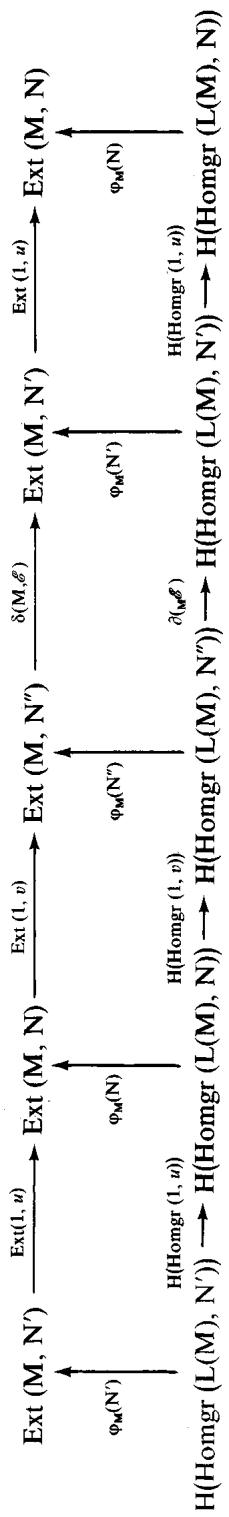
\includegraphics[keepaspectratio]{images/part001_97747f10.jpg}}

是 A-模的具有正合行的交换图。则 k-模的图

\[
\begin{array}{c} \operatorname{Ext} _ {\mathbf {A}} (\mathbf {M}, \mathbf {N} ^ {\prime \prime}) \xrightarrow {\delta (\mathbf {M} , \mathcal {E})} \operatorname{Ext} _ {\mathbf {A}} (\mathbf {M}, \mathbf {N} ^ {\prime}) \\ \operatorname{Ext} (f, g ^ {\prime \prime}) \Big | _ {\downarrow} \qquad \qquad \qquad \qquad \qquad \qquad \qquad \qquad \qquad \qquad \qquad \qquad \qquad \qquad \qquad \qquad \qquad \qquad \qquad \qquad \qquad \qquad \qquad \qquad \qquad \qquad \qquad \qquad \qquad \qquad \qquad \qquad \qquad \qquad \\ \operatorname{Ext} _ {\mathbf {A}} (\mathbf {M} _ {1}, \mathbf {N} _ {1} ^ {\prime \prime}) \xrightarrow {\delta (\mathbf {M} , \mathcal {E} _ {1})} \operatorname{Ext} _ {\mathbf {A}} (\mathbf {M} _ {1}, \mathbf {N} _ {1} ^ {\prime}) \end{array}
\]

是交换的。

这由 X，第 31 页，命题 2 应用于该交换图得出。

\[
\begin{array}{l} 0 \xrightarrow {\operatorname{Homgr} _ {A} (L (M) , N ^ {\prime})} \xrightarrow {\operatorname{Homgr} _ {A} (L (M) , N)} \xrightarrow {\operatorname{Homgr} _ {A} (L (M) , N ^ {\prime \prime})} 0 \\ \operatorname{Homgr} (L (f), g ^ {\prime}) \Big | _ {\downarrow} \quad \operatorname{Homgr} (1, u ^ {\prime}) \quad \Big | _ {\downarrow} \quad \operatorname{Homgr} (L (f), g) \quad \Big | _ {\downarrow} \quad \operatorname{Homgr} (L (f), g ^ {\prime \prime}) \\ 0 \xrightarrow {\operatorname{Homgr} _ {A} (L (M _ {1}) , N _ {1} ^ {\prime})} \xrightarrow {\operatorname{Homgr} _ {A} (L (M _ {1}) , N _ {1})} \xrightarrow {\operatorname{Homgr} _ {A} (L (M _ {1}) , N _ {1} ^ {\prime \prime})} 0 \end{array}
\]

设 N 是一个 A-模，且

\[
0 \rightarrow \mathbf {M} ^ {\prime} \xrightarrow {r} \mathbf {M} \xrightarrow {s} \mathbf {M} ^ {\prime \prime} \rightarrow 0\tag{$(\mathcal{F})$}
\]

一个 A-模的正合序列；复形序列

\[
\begin{array}{r l} (\mathcal {F} _ {\mathrm{N}}) & 0 \longrightarrow \operatorname{Homgr} _ {\mathrm{A}} (\mathrm{M} ^ {\prime \prime}, \mathrm{I} (\mathrm{N})) \xrightarrow {\operatorname{Homgr} (s , 1)} \operatorname{Homgr} _ {\mathrm{A}} (\mathrm{M}, \mathrm{I} (\mathrm{N})) \\ & \xrightarrow {\operatorname{Homgr} (r , 1)} \operatorname{Homgr} _ {\mathrm{A}} (\mathrm{M} ^ {\prime}, \mathrm{I} (\mathrm{N})) \longrightarrow 0 \end{array}
\]

是正合的（X，第 83 页，命题 2，a））；令

\[
\partial (\mathcal {F} _ {\mathrm{N}}): \mathrm{H} (\operatorname{Homgr} _ {\mathrm{A}} (\mathrm{M} ^ {\prime}, \mathrm{I} (\mathrm{N}))) \rightarrow \mathrm{H} (\operatorname{Homgr} _ {\mathrm{A}} (\mathrm{M} ^ {\prime \prime}, \mathrm{I} (\mathrm{N})))
\]

相应的连接同态。

定义3. --- 称相对于正合序列（\(\mathcal{F}\)）以及模 N 的扩张模的连接同态为复合同态

\[
\delta (\mathcal {F}, \mathrm{N}): \overline {{\varphi}} _ {\mathrm{N}} (\mathrm{M} ^ {\prime \prime}) \circ \partial (\mathcal {F} _ {\mathrm{N}}) \circ \overline {{\varphi}} _ {\mathrm{N}} (\mathrm{M} ^ {\prime}) ^ {- 1}: \operatorname{Ext} _ {\mathrm{A}} (\mathrm{M} ^ {\prime}, \mathrm{N}) \rightarrow \operatorname{Ext} _ {\mathrm{A}} (\mathrm{M} ^ {\prime \prime}, \mathrm{N}).
\]

这是一个 \(k\) -分次同态，其次数递增 1，其齐次分量记为 \(\delta^{n}(\mathcal{F}, \mathbf{N}) : \operatorname{Ext}_{\mathbf{A}}^{n}(\mathbf{M}', \mathbf{N}) \to \operatorname{Ext}_{\mathbf{A}}^{n+1}(\mathbf{M}'', \mathbf{N})\) .

然后我们如上证明以下命题：

定理2. —— k-模同态的右无界序列

\[
\begin{array}{r l} 0 & \xrightarrow {\quad} \operatorname{Hom} _ {A} (M ^ {\prime \prime}, N) \xrightarrow {\operatorname{Hom} (s , 1)} \operatorname{Hom} _ {A} (M, N) \xrightarrow {\operatorname{Hom} (r , 1)} \operatorname{Hom} _ {A} (M ^ {\prime}, N) \\ & \xrightarrow {\delta^ {\circ} (\mathcal {F} , N)} \operatorname{Ext} _ {A} ^ {1} (M ^ {\prime \prime}, N) \to \dots \xrightarrow {\delta^ {n - 1} (\mathcal {F} , N)} \operatorname{Ext} _ {A} ^ {n} (M ^ {\prime \prime}, N) \xrightarrow {\operatorname{Ext} ^ {n} (s , 1)} \operatorname{Ext} _ {A} ^ {n} (M, N) \\ & \xrightarrow {\operatorname{Ext} ^ {n} (r , 1)} \operatorname{Ext} _ {A} ^ {n} (M ^ {\prime}, N) \xrightarrow {\delta^ {n} (\mathcal {F} , N)} \operatorname{Ext} _ {A} ^ {n + 1} (M ^ {\prime \prime}, N) \to \dots \end{array}
\]

是正合的。

推论. —— 若 Ext \(_{A}^{1}\) (M'', N) = 0，序列

\[
0 \longrightarrow \operatorname{Hom} _ {\mathrm{A}} \left(\mathrm{M} ^ {\prime \prime}, \mathrm{N}\right) \xrightarrow {\operatorname{Hom} (s , 1)} \operatorname{Hom} _ {\mathrm{A}} (\mathrm{M}, \mathrm{N}) \xrightarrow {\operatorname{Hom} (r , 1)} \operatorname{Hom} _ {\mathrm{A}} \left(\mathrm{M} ^ {\prime}, \mathrm{N}\right) \longrightarrow 0
\]

是正合的。

命题 9. --- 设 \(g: \mathbf{N} \to \mathbf{N}_1\) 是 A-模的同态，且

\[
(\mathcal {F} _ {1})
\]

\[
0 \longrightarrow \mathbf {M} _ {1} ^ {\prime} \xrightarrow {r _ {1}} \mathbf {M} _ {1} \xrightarrow {s _ {1}} \mathbf {M} _ {1} ^ {\prime \prime} \longrightarrow 0
\]

\[
f ^ {\prime} \Big \downarrow \qquad f \Big \downarrow \qquad f ^ {\prime \prime} \Big \downarrow
\]

\[
0 \longrightarrow \mathbf {M} ^ {\prime} \stackrel {r} {\longrightarrow} \mathbf {M} \stackrel {s} {\longrightarrow} \mathbf {M} ^ {\prime \prime} \longrightarrow 0\tag{$(\mathcal{F})$}
\]

是 A-模的具有正合行的交换图。则 k-模的图

\[
\begin{array}{c} \operatorname{Ext} _ {\mathbf {A}} (\mathbf {M} ^ {\prime}, \mathbf {N}) \xrightarrow {\delta (\mathcal {F} , \mathbf {N})} \operatorname{Ext} _ {\mathbf {A}} (\mathbf {M} ^ {\prime \prime}, \mathbf {N}) \\ \operatorname{Ext} _ {\mathbf {A}} (f ^ {\prime}, g) \Big \downarrow \\ \operatorname{Ext} _ {\mathbf {A}} (\mathbf {M} _ {1} ^ {\prime}, \mathbf {N} _ {1}) \xrightarrow {\delta (\mathcal {F} _ {1} , \mathbf {N} _ {1})} \operatorname{Ext} _ {\mathbf {A}} (\mathbf {M} _ {1} ^ {\prime \prime}, \mathbf {N} _ {1}) \end{array}
\]

是交换的。

\subsection{投射模、内射模与扩张模}

命题10. —— 设 M 是一个 A-模。以下条件等价：

\begin{enumerate}
\def\labelenumi{(\roman{enumi})}
\item
  M 是投射的。
\item
  \(\operatorname{Ext}_{\mathbf{A}}^{i}(\mathbf{M},\mathbf{N}) = 0\) （对于每个 A-模 \(\mathbf{N}\) 以及每个整数 \(i > 0\)）.
\item
  \(\mathrm{Ext}_{\mathbf{A}}^{1}(\mathbf{M},\mathbf{N}) = 0\) （对于每个 A-模 \(\mathbf{N}\)）.
\item
  存在一个正合序列
\end{enumerate}

\[
0 \rightarrow \mathrm{K} \xrightarrow {u} \mathrm{P} \xrightarrow {r} \mathrm{M} \rightarrow 0,
\]

\(\text{其中 P 是投射的，且其中 } \text{ Ext}_{\mathbf{A}}^{1}(\mathbf{M}, \mathbf{K}) = 0.\)

\begin{enumerate}
\def\labelenumi{(\roman{enumi})}
\item
  \(\Rightarrow\) (ii)：这是 X 中命题 5 的推论，第 88 页。
\item
  \(\Rightarrow\) （iii）：这是平凡的。
\item
  \(\Rightarrow\) (iv)：这是显然的，因为 M 是自由模 P 的商模。
\item
  \(\Rightarrow\) (i)：由于 \(\operatorname{Ext}_{\mathbf{A}}^{1}(\mathbf{M},\mathbf{K}) = 0\) ，典范映射
\end{enumerate}

\[
\operatorname{Hom} _ {\mathbf {A}} (\mathbf {M}, \mathbf {P}) \rightarrow \operatorname{Hom} _ {\mathbf {A}} (\mathbf {M}, \mathbf {M})
\]

是满射（X，第 90 页，推论）；因此存在 v 的一个 A-线性截面，且 M 同构于 P 的一个直和项，从而是投射的。

命题11. --- 设 N 为一个 A-模。以下条件等价：

\begin{enumerate}
\def\labelenumi{(\roman{enumi})}
\item
  N 是内射的。
\item
  \(\operatorname{Ext}_{\mathbf{A}}^{i}(\mathbf{M},\mathbf{N}) = 0\) （对于每个 A-模 M 和每个整数 \(i > 0\)）.
\item
  \(\operatorname{Ext}_{\mathbf{A}}^{1}(\mathbf{M},\mathbf{N}) = 0\) （对于每个 A-模 \(\mathbf{M}\)）.
\item
  存在一个正合序列
\end{enumerate}

\[
0 \rightarrow \mathrm{N} \xrightarrow {u} \mathrm{I} \xrightarrow {v} \mathrm{C} \rightarrow 0,
\]

\(\text{其中 I 是内射的且其中 } \text{ Ext}_{\mathbf{A}}^{1} (\mathbf{C}, \mathbf{N}) = 0;\)

\begin{enumerate}
\def\labelenumi{(\alph{enumi})}
\setcounter{enumi}{21}
\item
  \(\operatorname{Ext}_{\mathbf{A}}^{1}(\mathbf{M},\mathbf{N}) = 0\) （对于每个单演 A-模 \(\mathbf{M}\)）.
\item
  \(\Rightarrow\) (ii)：这是 X 中命题 5 的推论，第 88 页。
\end{enumerate}

\begin{enumerate}
\def\labelenumi{(\roman{enumi})}
\setcounter{enumi}{1}
\item
  \(\Rightarrow\) (iii) \(\Rightarrow\) (v)：这是平凡的。
\item
  \(\Rightarrow\) (iv)：这是显然的，因为 N 是内射模的子模（X，第 19 页，推论 3）。
\item
  \(\Rightarrow\) (i)：由于 \(\operatorname{Ext}_{\mathbf{A}}^{1}(\mathbf{C},\mathbf{N}) = 0\) ，典范同态
\end{enumerate}

\[
\operatorname{Hom} _ {\mathbf {A}} (\mathrm{I}, \mathbf {N}) \rightarrow \operatorname{Hom} _ {\mathbf {A}} (\mathbf {N}, \mathbf {N})
\]

是满射的（X，第 93 页，推论）；因此存在 u 的一个 A-线性收缩，且 N 同构于 I 的一个直和项，从而 N 是内射的（X，第 16 页，命题 9）。

\begin{enumerate}
\def\labelenumi{(\alph{enumi})}
\setcounter{enumi}{21}
\tightlist
\item
  \(\Rightarrow\) (i)：若 a 是 A 的一个理想，则有 \(\operatorname{Ext}_{\mathbf{A}}^{1}(\mathbf{A}/\mathfrak{a},\mathbf{N})=0\) ；因此典范映射 \(\operatorname{Hom}_{\mathbf{A}}(\mathbf{A},\mathbf{N})\to\operatorname{Hom}_{\mathbf{A}}(\mathfrak{a},\mathbf{N})\) 是满射的，且 N 是内射的（X，第 16 页，命题 10）。
\end{enumerate}

\subsection{泛系数公式}

在本节中，我们考虑两个 A-模复形 (C, d) 和 (C', d')。考虑如下典范正合序列：

\[
0 \rightarrow \mathrm{Z} (\mathrm{C}) \stackrel {{j}} {{\rightarrow}} \mathrm{C} \stackrel {{\delta}} {{\rightarrow}} \mathrm{B} (\mathrm{C}) (- 1) \rightarrow 0,\tag{I}
\]

\((\mathrm{II}_{p})\)

\[
0 \to \mathrm{B} _ {p} (\mathrm{C}) \stackrel {{i}} {{\to}} \mathrm{Z} _ {p} (\mathrm{C}) \stackrel {{p}} {{\to}} \mathrm{H} _ {p} (\mathrm{C}) \to 0;
\]

我们从 δ 推出一个 k-同态

\[
\mathrm{H} (\text { Homgr } (\delta , 1)): \mathrm{H} (\text { Homgr } _ {\mathbf {A}} (\mathrm{B} (\mathbf {C}), \mathbf {C} ^ {\prime})) (1) \rightarrow \mathrm{H} (\text { Homgr } _ {\mathbf {A}} (\mathbf {C}, \mathbf {C} ^ {\prime}));
\]

由 \((\mathrm{II}_{p})\) 推出连接同态：

\[
\delta \left(\mathrm{II} _ {p}, \mathrm{H} ^ {q} \left(\mathrm{C} ^ {\prime}\right)\right): \operatorname{Hom} _ {\mathrm{A}} \left(\mathrm{B} _ {p} (\mathrm{C}), \mathrm{H} ^ {q} \left(\mathrm{C} ^ {\prime}\right)\right)\rightarrow \operatorname{Ext} _ {\mathrm{A}} ^ {1} \left(\mathrm{H} _ {p} (\mathrm{C}), \mathrm{H} ^ {q} \left(\mathrm{C} ^ {\prime}\right)\right).
\]

由此，通过过渡到乘积，得到 k-模的同态：

\[
\varphi^ {n}: \operatorname{Homgr} _ {\mathbf {A}} ^ {n} (\mathrm{B} (\mathrm{C}), \mathrm{H} (\mathrm{C} ^ {\prime})) \rightarrow \prod_ {p + q = n} \operatorname{Ext} _ {\mathbf {A}} ^ {1} \left(\mathrm{H} _ {p} (\mathrm{C}), \mathrm{H} ^ {q} (\mathrm{C} ^ {\prime})\right)
\]

还有典范同态（X，第 82 页）

\[
\lambda^ {n} (\mathrm{B} (\mathrm{C}), \mathrm{C} ^ {\prime}): \mathrm{H} ^ {n} \left(\operatorname{Homgr} _ {\mathrm{A}} (\mathrm{B} (\mathrm{C}), \mathrm{C} ^ {\prime})\right)\rightarrow \operatorname{Homgr} _ {\mathrm{A}} ^ {n} (\mathrm{B} (\mathrm{C}), \mathrm{H} (\mathrm{C} ^ {\prime})) .
\]

在这些记号下：

定理3. --- 假设 A-模 B(C) 和 Z(C) 是投射的。那么对每个 n，存在唯一的 k-模同态

\[
\beta^ {n}: \prod_ {p + q = n - 1} \operatorname{Ext} _ {\mathbf {A}} ^ {1} \left(\mathrm{H} _ {p} (\mathbf {C}), \mathrm{H} ^ {q} \left(\mathbf {C} ^ {\prime}\right)\right)\rightarrow \mathrm{H} ^ {n} \left(\operatorname{Homgr} _ {\mathbf {A}} \left(\mathrm{C}, \mathrm{C} ^ {\prime}\right)\right)
\]

从而使得图表交换

\[
\begin{array}{c} \operatorname{Homgr} _ {\mathbf {A}} ^ {n - 1} (\mathrm{B} (\mathrm{C}), \mathrm{H} (\mathrm{C} ^ {\prime})) \xleftarrow {\lambda^ {n - 1} (\mathrm{B} (\mathrm{C}) , \mathrm{C} ^ {\prime})} \mathrm{H} ^ {n - 1} (\operatorname{Homgr} _ {\mathbf {A}} (\mathrm{B} (\mathrm{C}), \mathrm{C} ^ {\prime})) \\ \prod_ {p + q = n - 1} \operatorname{Ext} _ {\mathbf {A}} ^ {1} (\mathrm{H} _ {p} (\mathrm{C}), \mathrm{H} ^ {q} (\dot {\mathrm{C}} ^ {\prime})) \xrightarrow {\beta^ {n}} \mathrm{H} ^ {n} (\operatorname{Homgr} _ {\mathbf {A}} (\mathrm{C}, \mathrm{C} ^ {\prime})). \end{array}
\]

分次 k-模的序列

\[
\begin{array}{r l} 0 \longrightarrow & \prod_ {p + q = n - 1} \operatorname{Ext} _ {\mathrm{A}} ^ {1} \left(\mathrm{H} _ {p} (\mathrm{C}), \mathrm{H} ^ {q} (\mathrm{C} ^ {\prime})\right) \xrightarrow {\beta^ {n}} \mathrm{H} ^ {n} \big (\mathrm{Homg} _ {\mathrm{A}} (\mathrm{C}, \mathrm{C} ^ {\prime}) \big) \\ & \xrightarrow {\lambda^ {n} (\mathrm{C} , \mathrm{C} ^ {\prime})} \prod_ {p + q = n} \mathrm{Hom} _ {\mathrm{A}} \left(\mathrm{H} _ {p} (\mathrm{C}), \mathrm{H} ^ {q} (\mathrm{C} ^ {\prime})\right) \to 0 \end{array}\tag{11}
\]

是正合的。

注记. --- 可以证明一个类似的命题，假设 \(\mathbf{B}_{n}(\mathbf{C}')\) 和 \(\mathbf{C}'/\mathbf{B}_{n}(\mathbf{C}')\) 对每个 n 都是内射的。

为简单起见，设 \(\mathbf{B} = \mathbf{B}(\mathbf{C}), \mathbf{Z} = \mathbf{Z}(\mathbf{C}), \mathbf{H} = \mathbf{H}(\mathbf{C})\) 和 \(\mathbf{H}' = \mathbf{H}(\mathbf{C}')\) 。由于 B 是投射的，由 (I) 可导出一个正合序列

\[
\begin{array}{r l}(1 2) \quad&0 \rightarrow \operatorname{Homgr} _ {\mathbf {A}} (\mathrm{B}, \mathrm{C} ^ {\prime}) (1) \xrightarrow {\operatorname{Homgr} (\delta , 1)} \operatorname{Homgr} _ {\mathbf {A}} (\mathrm{C}, \mathrm{C} ^ {\prime})\\&\xrightarrow {\operatorname{Homgr} (j , 1)} \operatorname{Homgr} _ {\mathbf {A}} (\mathrm{Z}, \mathrm{C} ^ {\prime}) \rightarrow 0.\end{array}
\]

引理2. --- 连接同态

\[
\mathrm{H} ^ {n} \left(\operatorname{Homgr} _ {\mathbf {A}} \left(\mathrm{Z}, \mathrm{C} ^ {\prime}\right)\right)\rightarrow \mathrm{H} ^ {n} \left(\operatorname{Homgr} _ {\mathbf {A}} \left(\mathrm{B}, \mathrm{C} ^ {\prime}\right)\right)
\]

与 (12) 相关联的连接同态等于 \((-1)^{n+1}\) H(Homgr(i, 1)).

事实上，设 \(a \in \mathbf{Z}^n(\text{Homgr}_A(Z, C'))\) ；这是一个次数递增 \(n\) 的、从 \(Z\) 到 \(C'\) 的复形态射，其值因此位于 \(Z(C')\) 中。由于正合序列 (I) 是分裂的（因为 B 是投射的）， \(a\) 延拓为一个元素 \(b\) ，它属于 \(\text{Homgr}_A^n(C, Z(C'))\) 。根据定义， \(a\) 的类在该连接同态下的像是 \(H^n(\text{Homgr}_A(B, C'))\) 中同态 \(u\) （从 \(B(C)\) 到 \(C'\) ）的类，使得对于 \(x \in C\) ，有

\[
u (d x) = \mathrm{D} b (x) = d ^ {\prime} b (x) - (- 1) ^ {n} b (d x) = (- 1) ^ {n + 1} b (d x) = (- 1) ^ {n + 1} a (d x),
\]

由此得出断言。

因此，与（12）相关联的同调正合列给出如下正合序列

\[
\rightarrow \mathrm{H} ^ {n} (\operatorname{Homgr} _ {\mathrm{A}} (Z, C ^ {\prime})) \xrightarrow {\mathrm{H} (\operatorname{Homgr} (i , 1))} \mathrm{H} ^ {n} (\operatorname{Homgr} _ {\mathrm{A}} (B, C ^ {\prime}))
\]

\[
\xrightarrow {\mathrm{H} (\text { Homgr } (\delta , 1))} \mathrm{H} ^ {n + 1} \left(\text { Homgr } _ {\mathrm{A}} \left(\mathrm{C}, \mathrm{C} ^ {\prime}\right)\right) \xrightarrow {\mathrm{H} (\text { Homgr } (j , 1))} \mathrm{H} ^ {n + 1} \left(\text { Homgr } _ {\mathrm{A}} \left(\mathrm{Z}, \mathrm{C} ^ {\prime}\right)\right)\rightarrow \dots .
\]

此外，由于 Z 是投射的，由 \((II_{p})\) 可导出正合序列

\[
0 \to \mathrm{Hom} _ {\mathbf {A}} (\mathrm{H} _ {p}, \mathrm{H} ^ {\prime q}) \to \mathrm{Hom} _ {\mathbf {A}} (Z _ {p}, \mathrm{H} ^ {\prime q}) \to \mathrm{Hom} _ {\mathbf {A}} (\mathrm{B} _ {p}, \mathrm{H} ^ {\prime q}) \to \mathrm{Ext} _ {\mathbf {A}} ^ {1} (\mathrm{H} _ {p}, \mathrm{H} ^ {\prime q}) \to 0,
\]

由此，通过取乘积，得到正合序列

\[
\begin{array}{r l} 0 \to \operatorname{Homgr} _ {\mathbf {A}} ^ {n} (\mathbf {H}, \mathbf {H} ^ {\prime}) & \to \operatorname{Homgr} _ {\mathbf {A}} ^ {n} (Z, \mathbf {H} ^ {\prime}) \to \operatorname{Homgr} _ {\mathbf {A}} ^ {n} (\mathbf {B}, \mathbf {H} ^ {\prime}) \\ & \to \prod_ {p + q = n} \operatorname{Ext} _ {\mathbf {A}} ^ {1} (\mathbf {H} _ {p}, \mathbf {H} ^ {\prime q}) \to 0. \end{array}
\]

最后，有第 1 号中的典范同态：

\[
\begin{array}{l} \lambda_ {\mathrm{B}} = \lambda (\mathrm{B}, \mathrm{C} ^ {\prime}): \mathrm{H} (\mathrm{Homgr} _ {\mathrm{A}} (\mathrm{B}, \mathrm{C} ^ {\prime})) \to \mathrm{Homgr} _ {\mathrm{A}} (\mathrm{B}, \mathrm{H} ^ {\prime}), \\ \lambda_ {\mathrm{Z}} = \lambda (\mathrm{Z}, \mathrm{C} ^ {\prime}): \mathrm{H} (\mathrm{Homgr} _ {\mathrm{A}} (\mathrm{Z}, \mathrm{C} ^ {\prime})) \to \mathrm{Homgr} _ {\mathrm{A}} (\mathrm{Z}, \mathrm{H} ^ {\prime}), \\ \lambda_ {\mathrm{C}} = \lambda (\mathrm{C}, \mathrm{C} ^ {\prime}): \mathrm{H} (\mathrm{Homgr} _ {\mathrm{A}} (\mathrm{C}, \mathrm{C} ^ {\prime})) \to \mathrm{Homgr} _ {\mathrm{A}} (\mathrm{H}, \mathrm{H} ^ {\prime}), \end{array}
\]

由此得到 X 第 97 页上的行正合图表。

该图表由 \(\lambda\) 同态的构造是交换的。此外，由于复形 B 和 Z 是分裂且投射的， \(\lambda_{\mathrm{B}}\) 和 \(\lambda_{\mathrm{Z}}\) 是双射的（X，第 84 页，推论 1）。由此一方面可推出， \(\lambda_{\mathrm{C}}^{n}\) 是满射的，其核等于 Im H \(^{n}\) (Homgr ( \(\delta\) , 1))，另一方面可推出， \(\varphi^{n-1} \circ \lambda_{\mathrm{B}}^{n-1}\) 是满射的，其核等于 Ker H \(^{n}\) (Homgr ( \(\delta\) , 1))。定理由此立即得出。

推论 1. --- 假设 B(C) 和 Z(C) 是投射的，且 B \(^{n}\) (C') 对每个 n 都是内射的。则正合序列 (11) 是分裂的。

这由定理及以下引理得出：

引理 3. --- 若 B(C) 是投射的且 \(\mathbf{B}_{n}(\mathbf{C}^{\prime})\) 对每个 \(n\) ，典范同态 \(\lambda(\mathbf{C}, \mathbf{C}^{\prime}): \mathrm{H}(\mathrm{Homgr}_{\mathbf{A}}(\mathbf{C}, \mathbf{C}^{\prime})) \to \mathrm{Homgr}_{\mathbf{A}}(\mathrm{H}(\mathbf{C}), \mathrm{H}(\mathbf{C}^{\prime}))\) 有一个 \(k\) -线性截面。

事实上，根据 X，第 35 页，注记 a) 和 b)，存在拟同构

\[
\varphi : \mathrm{C} \rightarrow \mathrm{H} (\mathrm{C}) \quad \text { and } \quad \varphi^ {\prime}: \mathrm{H} (\mathrm{C} ^ {\prime}) \rightarrow \mathrm{C} ^ {\prime}
\]

使得 \(\mathbf{H}(\varphi) = 1_{\mathbf{H}(\mathbf{C})}\) 和 \(\bar{\mathbf{H}} (\varphi^{\prime}) = 1_{\mathbf{H}(\mathbf{C}^{\prime})}\) .

在交换图中

\[
\begin{array}{l} \mathrm{H} (\operatorname{Homgr} _ {\mathbf {A}} (\mathrm{H} (\mathrm{C}), \mathrm{H} (\mathrm{C} ^ {\prime})) \xrightarrow {\mathrm{H} (\operatorname{Homgr} (\varphi , \varphi^ {\prime}))} \mathrm{H} (\operatorname{Homgr} _ {\mathbf {A}} (\mathrm{C}, \mathrm{C} ^ {\prime})) \\ \lambda (\mathrm{H} (\mathrm{C}), \mathrm{H} (\mathrm{C} ^ {\prime})) \Big | _ {\downarrow} \\ \operatorname{Homgr} _ {\mathbf {A}} (\mathrm{H} (\mathrm{C}), \mathrm{H} (\mathrm{C} ^ {\prime})) \xrightarrow {\operatorname{Homgr} (\mathrm{H} (\varphi) , \mathrm{H} (\varphi^ {\prime}))} \operatorname{Homgr} _ {\mathbf {A}} (\mathrm{H} (\mathrm{C}), \mathrm{H} (\mathrm{C} ^ {\prime}))  , \end{array}
\]

\(\lambda(H(C), H(C'))\) 是双射且 Homgr \((H(\varphi), H(\varphi'))\) 是恒等映射，由此得出断言。

Homgr \(^{n-1}\) (Z, H') → Homgr \(^{n-1}\) (B, H') → Φ \(^{n-1}\) → Πp+q=n-1 Ext \(^{1}\) (Hp, H'q) → 0

H \(^{n-1}\) (Homgr(A, C')) → H \(^{n-1}\) (Homgr(A, B, C')) → H \(^{n}\) (Homgr(A, C)) → H \(^{n}\) (Homgr(A, C)) → H \(^{n}\) (Homgr(A, B, C))

0 → Homgr \(^{n}\) (H, H') → Homgr \(^{n}\) (Z, H') → Homgr \(^{n}\) (B, H')

推论 2. --- 若 B(C) 和 Z(C) 是投射的，则对每个 A-模 N 和每个整数 n，存在一个分裂的正合序列：

\[
(1 3) \quad 0 \longrightarrow \operatorname{Ext} _ {\mathbf {A}} ^ {1} \left(\mathrm{H} _ {n - 1} (\mathrm{C}), \mathrm{N}\right) \xrightarrow {\beta^ {n}} \mathrm{H} ^ {n} \left(\operatorname{Homgr} _ {\mathbf {A}} (\mathrm{C}, \mathrm{N})\right) \xrightarrow {\lambda^ {n}} \operatorname{Hom} _ {\mathbf {A}} \left(\mathrm{H} _ {n} (\mathrm{C}), \mathrm{N}\right) \longrightarrow 0.
\]

推论 3（“泛系数公式”）. --- 设 A 是主理想环且 C 是自由的。则对每个 A-模 N 和每个整数 n，存在一个分裂的正合序列 (13)。

事实上，B(C) 和 Z(C) 作为自由模 C 的子模是自由的（VII，§ 3，定理 1 的推论 2）。

推论 4. --- 若 C 右有界且 C 和 H(C) 是投射的，则

\[
\lambda (C, C ^ {\prime}): H \left(\operatorname{Homgr} _ {A} (C, C ^ {\prime})\right)\rightarrow \operatorname{Homgr} _ {A} \left(H (C), H \left(C ^ {\prime}\right)\right)
\]

是双射。

由定理可知，只需证明 B(C) 和 Z(C) 是投射的。现在我们有正合序列

\[
\begin{array}{l} 0 \to \mathrm{B} _ {n} (\mathrm{C}) \to Z _ {n} (\mathrm{C}) \to \mathrm{H} _ {n} (\mathrm{C}) \to 0 \\ 0 \to Z _ {n} (\mathrm{C}) \to \mathrm{C} _ {n} \to \mathrm{B} _ {n - 1} (\mathrm{C}) \to 0, \end{array}
\]

因此 \((\mathbf{B}_{n - 1}(\mathbf{C})\) 是投射的) \(\Rightarrow (\mathbf{Z}_n(\mathbf{C})\) 是投射的) \(\Rightarrow (\mathbf{B}_n(\mathbf{C})\) 是投射的)。我们通过指出 \(\mathbf{B}_n(\mathbf{C}) = 0\) （对足够小的 \(n\) ）来结束。

\subsection{推广到多模复形；典范同构}

设 B, B' 为两个环，C 为 (A, B)-双模复形，C' 为 (A, B')-双模复形；则 (Homgr\_A (C, C′), D) 是 (B, B′)-双模复形，且典范同态 \(\lambda: H(\text{Homgr}_A (\text{C}, \text{C'})) \to \text{Homgr}_A (\text{H}(\text{C}), \text{H}(\text{C'}))\) 是 (B, B')-双模同态。

若 M 是 (A, B)-双模，N 是 (A, B')-双模，则 Homgr \(_{A}\) (L(M), I(N)) 是 (B, B')-双模复形，因此 Ext \(_{A}\) (M, N) 具有自然的分次 (B, B')-双模结构；在次数 0 项上，该结构与 Hom \(_{A}\) (M, N) 的结构一致（II，第 35 页）。

若 \(\lambda\in\mathbf{B},\lambda^{\prime}\in\mathbf{B}^{\prime}\) 并且如果我们记 \(\lambda_{\mathrm{M}},\lambda_{\mathrm{N}}^{\prime},\lambda_{\mathrm{E}},\lambda_{\mathrm{E}}^{\prime}\) 为位似 \(x\mapsto x\lambda,y\mapsto y\lambda^{\prime},z\mapsto\lambda z,z\mapsto z\lambda^{\prime}\) ，它们分别是 M, N, Ext \(_{\mathrm{A}}\) (M, N), Ext \(_{\mathrm{A}}\) (M, N) 的，则我们有

\[
\lambda_ {\mathrm{E}} = \operatorname{Ext} _ {\mathbf {A}} \left(\lambda_ {\mathbf {M}}, 1\right), \quad \lambda_ {\mathrm{E}} ^ {\prime} = \operatorname{Ext} \left(1, \lambda_ {\mathbf {N}} ^ {\prime}\right),
\]

这给出了 Ext \(_{A}\) (M, N) 的双模结构的另一种描述。我们把第 4 号和第 6 号推广到多模复形的情形留给读者。

设 C, C′ 和 C′′ 是 A-模的复形。映射的复合定义了一个次数为零的分次同态：

\[
\operatorname{Homgr} _ {\mathbf {A}} \left(\mathrm{C} ^ {\prime}, \mathrm{C} ^ {\prime \prime}\right) \otimes_ {k} \operatorname{Homgr} _ {\mathbf {A}} \left(\mathrm{C}, \mathrm{C} ^ {\prime}\right)\rightarrow \operatorname{Homgr} _ {\mathbf {A}} \left(\mathrm{C}, \mathrm{C} ^ {\prime \prime}\right).\tag{14}
\]

设 B、B'、E 为环，C、C'、C'' 分别为 (B', A)-双模、(A, E)-双模、(B, E)-双模的复形。通过限制 II 第 73 页的典范同构，得到 (B, B')-双模的一个双射同态：

\[
\operatorname{Homgr} _ {E} \left(C \otimes_ {A} C ^ {\prime}, C ^ {\prime \prime}\right)\rightarrow \operatorname{Homgr} _ {A} \left(C, \operatorname{Homgr} _ {E} \left(C ^ {\prime}, C ^ {\prime \prime}\right)\right).\tag{15}
\]

最后，设 B 为一个环，C 为右 B-模的复形，C' 为右 A-模的复形，C'' 为 (B, A)-双模的复形。我们由典范同态（II，第 75 页）推出

\[
\mathrm{C} _ {p} \otimes_ {\mathrm{B}} \operatorname{Hom} _ {\mathrm{A}} \left(\mathrm{C} _ {q} ^ {\prime}, \mathrm{C} _ {r} ^ {\prime \prime}\right)\rightarrow \operatorname{Hom} _ {\mathrm{A}} \left(\mathrm{C} _ {q} ^ {\prime}, \mathrm{C} _ {p} \otimes_ {\mathrm{B}} \mathrm{C} _ {r} ^ {\prime \prime}\right)
\]

一个次数为零的分次同态：

\[
\mathrm{C} \otimes_ {\mathrm{B}} \operatorname{Homgr} _ {\mathrm{A}} \left(\mathrm{C} ^ {\prime}, \mathrm{C} ^ {\prime \prime}\right)\rightarrow \operatorname{Homgr} _ {\mathrm{A}} \left(\mathrm{C} ^ {\prime}, \mathrm{C} \otimes_ {\mathrm{B}} \mathrm{C} ^ {\prime \prime}\right).\tag{16}
\]

当 C 是有限生成投射模时，此同态是双射的（II，第 75 页，命题 2）。

命题12.——同态（14）、（15）、（16）是复形的态射。

我们来证明它，例如对于同态（14）。记

\[
\kappa : \operatorname{Homgr} _ {\mathbf {A}} \left(\mathrm{C} ^ {\prime}, \mathrm{C} ^ {\prime \prime}\right) \otimes_ {k} \operatorname{Homgr} _ {\mathbf {A}} \left(\mathrm{C}, \mathrm{C} ^ {\prime}\right)\rightarrow \operatorname{Homgr} _ {\mathbf {A}} \left(\mathrm{C}, \mathrm{C} ^ {\prime \prime}\right)
\]

这个同态。设 \(f \in \operatorname{Homgr}_{\mathbf{A}}(\mathbf{C}', \mathbf{C}^{\prime})_{p}\) 和 \(g \in \operatorname{Homgr}_{\mathbf{A}}(\mathbf{C}, \mathbf{C}^{\prime})_{q}\) ；于是根据定义我们有 \(\kappa(f \otimes g) = f \circ g\) 。此外：

\[
\begin{array}{r l} \mathrm{D} (f \otimes g) = & \mathrm{D} f \otimes g + (- 1) ^ {p} f \otimes \mathrm{D} g = (d ^ {\prime \prime} \circ f) \otimes g - (- 1) ^ {p} (f \circ d ^ {\prime}) \otimes g + \\ & + (- 1) ^ {p} f \otimes (d ^ {\prime} \circ g) - (- 1) ^ {p + q} f \otimes (g \circ d), \end{array}
\]

由此可得

\[
\begin{array}{r l} & {\kappa \big (\mathbf {D} (f \otimes g) \big) = d ^ {\prime \prime} \circ f \circ g - (- 1) ^ {p} f \circ d ^ {\prime} \circ g +} \\ & {\qquad + (- 1) ^ {p} f \circ d ^ {\prime} \circ g - (- 1) ^ {p + q} f \circ g \circ d} \\ & {\qquad = d ^ {\prime \prime} \circ f \circ g - (- 1) ^ {p + q} f \circ g \circ d = \mathbf {D} (f \circ g) = \mathbf {D} \big (\kappa (f \otimes g) \big).} \end{array}
\]

类似地可证明同态(15)和(16)是复形的态射。

由态射 (14) 我们推出 \(k\) -模的同态（X，第 62 页）

\[
\mathrm{H} ^ {p} \left(\operatorname{Homgr} _ {\mathbf {A}} \left(\mathrm{C} ^ {\prime}, \mathrm{C} ^ {\prime \prime}\right)\right) \otimes_ {k} \mathrm{H} ^ {q} \left(\operatorname{Homgr} _ {\mathbf {A}} \left(\mathrm{C}, \mathrm{C} ^ {\prime}\right)\right)\rightarrow \mathrm{H} ^ {p + q} \left(\operatorname{Homgr} _ {\mathbf {A}} \left(\mathrm{C}, \mathrm{C} ^ {\prime \prime}\right)\right). \tag {17}
\]

取 C = A，我们看到同态：

\[
\operatorname{Homgr} _ {\mathbf {A}} \left(\mathrm{C} ^ {\prime}, \mathrm{C} ^ {\prime \prime}\right) \otimes_ {k} \mathrm{C} ^ {\prime} \rightarrow \mathrm{C} ^ {\prime \prime}\tag{18}
\]

它把 \(f \otimes x\) 映到 \(f(x)\) ，是左 A-模复形的一个态射；与之相伴的是分次 A-模的一个典范同态（X，第 80 页） \(\gamma : \mathrm{H}(\mathrm{Homgr}_{\mathbf{A}}(\mathbf{C}', \mathbf{C}')) \otimes_k \mathrm{H}(\mathbf{C}') \to \mathrm{H}(\mathbf{C}'')\) ，它对应于 \(k\) -模的典范同态

\[
\lambda : \mathrm{H} (\operatorname{Homgr} _ {\mathbf {A}} \left(\mathrm{C} ^ {\prime}, \mathrm{C} ^ {\prime \prime}\right)) \rightarrow \operatorname{Homgr} _ {\mathbf {A}} \left(\mathrm{H} (\mathrm{C} ^ {\prime}), \mathrm{H} (\mathrm{C} ^ {\prime \prime})\right).
\]

\section{非典范分解的使用}

我们沿用 § 4 的约定。
